% ======================================================================
%                  CONCLUSIONES Y RECOMENDACIONES
% ======================================================================
\chapter*{CONCLUSIONES Y RECOMENDACIONES}
\addcontentsline{toc}{chapter}{CONCLUSIONES Y RECOMENDACIONES}\label{cap:conclusiones}

\section*{Conclusiones}

\begin{enumerate}
\item Los planes de tiempo fijo o con
adaptación limitada no representan adecuadamente las variaciones direccionales de demanda, mientras que una
arquitectura exclusivamente remota introduce dependencia de la conectividad y un punto único de falla. Esto
justifica un módulo local complementario y no el reemplazo directo del controlador semafórico (OE1, OE2).

\item El diseño conceptual estableció una cadena trazable entre necesidades, requerimientos, funciones y
alternativas. La evaluación técnico-económica seleccionó el concepto cámara + procesamiento en el borde +
ICV + control difuso + nube segura + gabinete modular, principalmente por su autonomía local, su
interpretabilidad y su compatibilidad con una validación reproducible (OE3).

\item El diseño electrónico definió y dimensionó las funciones de sensado, procesamiento, comunicación,
alimentación, protección, respaldo y diagnóstico. El balance de potencia (consumo cercano a 145.7~W,
elevado a 182~W con un factor de seguridad), el dimensionamiento de las fuentes, la autonomía del
respaldo ($\sim$72~min) y la coordinación de protecciones quedaron resueltos a nivel de diseño; su cierre
para fabricación requiere la confirmación con componentes físicos (OE4).

\item El diseño mecánico incorporó gabinete, distribución interna, ventilación, acceso de mantenimiento y
soporte de cámara. El análisis estructural por elementos finitos arrojó un factor de seguridad mínimo de
5.94 y un desplazamiento máximo de 0.21~mm bajo la carga de viento de diseño, y el análisis térmico estimó
un incremento de 2.5~\textdegree C; la clasificación IP, la resistencia al vandalismo y el comportamiento
térmico en campo deben confirmarse mediante prototipo y ensayos (OE5).

\item El control difuso local se definió como núcleo por su interpretabilidad y su capacidad de operar en el
borde. Las entradas, las funciones de pertenencia, las reglas, la inferencia, la defuzzificación y las
saturaciones permiten revisar el comportamiento antes de emitir una recomendación. Ante una falla del
sensado o del módulo, la arquitectura inhibe la adaptación y conserva el plan seguro del controlador, que
mantiene la autoridad final sobre la actuación (OE6).

\item La elección de una cámara orientable se justifica como una estrategia de \emph{percepción activa}, en
la que el campo visual se dirige hacia el eje de mayor relevancia operacional del ciclo semafórico. Esta
decisión integra mecánica, electrónica, percepción y control local en un mismo módulo, y se
acompaña de una política de validez temporal (estados \textit{MOVING}/\textit{SETTLING}/\textit{OBSERVING} y
vigencia $T_{valid}$) que evita que la reorientación degrade la recomendación; la salida del sistema permanece
como recomendación y no como actuación directa sobre las luces (OE5, OE6).

\item La nube se delimitó como soporte para telemetría, históricos, alertas, coordinación y distribución
autorizada de parámetros, demostrándose que la decisión local continúa sin conectividad externa. La
ciberseguridad propuesta incorpora autenticación, cifrado, control de acceso por roles, validación de
parámetros, registro de eventos y mínimo privilegio; estas medidas son criterios de diseño y no equivalen a
una auditoría o certificación (OE7, OE8).

\item La verificación en SUMO comparó el control de tiempo fijo con el control difuso adaptativo en el
escenario de alta demanda de Lima-Centro, bajo condiciones comunes y con \textbf{30 semillas}, conservando el
mismo presupuesto de verde por ciclo. El control difuso redujo la demora media de 509.3 a 470.8~s/veh
($-7.6$~\%) y la saturación de cola en $4.2$~\%, disminuyó el índice de congestión de 0.506 a 0.494
($-2.4$~\%) e incrementó la velocidad media en $1.8$~\% y el \textit{throughput} en $3.1$~\%, manteniendo en
todo momento los límites duros de verde $[10,120]$~s. Todas las mejoras son estadísticamente significativas
(prueba t, $p<0.001$) y consistentes: el difuso supera al plan fijo en 28 de 30 semillas. La mejora no es
universal —en 2 de 30 réplicas el plan fijo iguala o supera al difuso—, lo que se reporta de forma explícita.
Frente a líneas base más exigentes en sensado (actuado, Webster, Max-Pressure), el difuso obtiene una mejora
bruta menor, pero es el único que opera con una sola cámara orientable, es interpretable y tolera la pérdida
de enlace. Estos resultados verifican el núcleo de control y acotan honestamente su alcance (OE9).

\item El análisis económico preliminar separó CAPEX y OPEX y situó el costo del primer año en torno a
S/~17~mil por intersección, dominado por la estructura mecánica y el sistema de visión. Antes de defender
una cifra definitiva deben actualizarse cotizaciones, tipo de cambio, consumo real y prorrateo de los
servicios de nube; la certificación, la obra civil y el piloto deben presupuestarse como etapas posteriores
(OE10).

\item La principal limitación del trabajo es la ausencia de fabricación, de calibración con aforos reales,
de integración con un controlador comercial certificado, de prueba vial y de auditoría de ciberseguridad.
Estas limitaciones no invalidan el diseño, pero restringen la generalización de los resultados a las
condiciones simuladas y a los supuestos documentados.

\item La arquitectura resultante constituye una base técnica trazable para un prototipo de laboratorio y un
piloto progresivo. La condición de avance debe ser demostrar cada requerimiento mandatorio en banco,
preservar la autoridad final del controlador y obtener la aprobación normativa e institucional antes de
cualquier intervención en vía pública.
\end{enumerate}

\section*{Recomendaciones}

\begin{itemize}
\item Fabricar un prototipo del módulo y verificar consumo, temperatura, respaldo, comunicaciones y
\textit{watchdog} en un banco de pruebas.
\item Probar la cámara con video real de Lima en condiciones de día, noche, contraluz, lluvia y neblina
costera, y medir la precisión de conteo, cola y velocidad.
\item Validar experimentalmente en prototipo la política de orientación de la cámara: tiempos de giro,
ventana de estabilización, precisión de posicionamiento, efecto de las vibraciones sobre la detección,
umbrales de confianza visual y desempeño ante oclusiones e iluminación variable. Comparar además, en
trabajos posteriores, la cámara orientable frente a una arquitectura multicámara bajo métricas de
cobertura, confiabilidad, latencia y robustez.
\item Calibrar la demanda y el comportamiento vehicular de SUMO con aforos reales, ampliar el número de
semillas y publicar los archivos de configuración y de salida para garantizar la reproducibilidad.
\item Integrar el módulo a un controlador semafórico comercial en un banco \textit{hardware-in-the-loop},
sin conexión directa a las lámparas durante la etapa inicial.
\item Ejecutar pruebas autorizadas de ciberseguridad: gestión de certificados, rotación de credenciales,
restauración de respaldos y respuesta ante incidentes.
\item Revisar la normativa vial, la seguridad funcional, la compatibilidad electromagnética, la protección
ambiental y los procedimientos municipales aplicables.
\item Realizar un piloto controlado en una intersección o recinto cerrado, con plan de reversión,
supervisión humana y métricas acordadas.
\item Mantener el aprendizaje por refuerzo, la predicción CNN--LSTM, la optimización metropolitana y la
detección de vehículos de emergencia como líneas futuras, hasta disponer de datos, validación fuera de
muestra y criterios de aceptación (Anexo~E).
\item Extender el estudio de una intersección a un corredor solo después de demostrar estabilidad local,
interoperabilidad y un beneficio estadísticamente sustentado.
\end{itemize}

% ======================================================================
%                            ANEXOS
% ======================================================================
\chapter*{ANEXOS}\addcontentsline{toc}{chapter}{ANEXOS}\label{anexos}

\noindent Los archivos de programación, simulación, esquemas CAD y recursos complementarios se conservan
como material digital de soporte de la tesis. A continuación se incluyen los anexos referenciados a lo largo
del documento.

% ---------------------------------------------------------------------
\section*{ANEXO A: Lista de requerimientos}
\addcontentsline{toc}{section}{ANEXO A: Lista de requerimientos}\label{anexo:requerimientos}

A partir de las necesidades del sistema se derivan los requerimientos, clasificados como exigencias
(obligatorias) o deseos (mejoras adicionales). La Tabla~\ref{tab:exigencias} resume las exigencias y deseos
por dominio de diseño, conforme a la estructura VDI 2221.

Para conducir el diseño y cerrar la validación, las exigencias anteriores se traducen en una
\textbf{especificación verificable codificada} (Tabla~\ref{tab:req-verificables}), donde cada requerimiento
recibe un código, un valor objetivo, su justificación y el método de verificación previsto. La
prioridad se clasifica como M (mandatoria), A (alta) o D (deseable). Esta tabla presenta la versión
consolidada que gobierna el resto de la tesis.

\begin{table}[H]
  \centering
  \footnotesize
  \caption{Resumen de exigencias y deseos por dominio de diseño.}
  \label{tab:exigencias}
  \begin{tabularx}{\linewidth}{@{}>{\raggedright\arraybackslash}p{2.6cm}>{\raggedright\arraybackslash}p{1.9cm}>{\raggedright\arraybackslash}X@{}}
    \toprule
    \textbf{Aspecto} & \textbf{Carácter} & \textbf{Especificación}\\
    \midrule
    Función principal & Exigencia & Sistema de semaforización adaptativa que optimiza la gestión del tráfico en
    tiempo real usando sensado IoT, comunicación con la nube y control inteligente interpretable basado en
    lógica difusa.\\
    Energía & Exigencia & Alimentación principal desde la red eléctrica (DC de 12\,V o 24\,V) con respaldo
    capaz de operar un mínimo de 1\,h ante corte de energía.\\
    Fuerzas & Exigencia & La estructura debe soportar el peso de placa, microcontrolador, sensores, actuadores
    y de la propia carcasa.\\
    Materia & Exigencia & Módulo resistente a temperatura, humedad, polvo y radiación solar; impermeable,
    antivandálico y con aislamiento contra cortocircuitos y daños físicos.\\
    Comunicación & Exigencia & Comunicación NTCIP entre semáforos y la plataforma centralizada, con base de
    datos para registro y análisis.\\
    Control & Exigencia & Control adaptativo que ajusta los ciclos según el tráfico en tiempo real, escalable a
    futuras intersecciones e integrando aprendizaje para mejorar la predicción de flujo.\\
    Software & Exigencia & Gestión de algoritmos de control adaptativo, procesamiento de sensores en tiempo
    real, actualización remota por la nube y ciberseguridad según estándares internacionales.\\
    Uso & Exigencia & Interoperabilidad con los semáforos y controladores existentes en Lima.\\
    Seguridad & Exigencia & Ciberseguridad según IEC 62443 y protección física del módulo frente a clima
    extremo y vandalismo (IP65).\\
    Geometría & Deseo & Módulo IoT de tamaño máximo aproximado de 70$\times$70$\times$80\,cm.\\
    Precio & Deseo & Solución de bajo costo, con presupuesto máximo estimado de 10\,000 soles por intersección.\\
    \bottomrule
  \end{tabularx}
  \fuente{Elaboración propia.}
\end{table}

\begin{landscape}
\footnotesize
\begin{longtable}{@{}p{1.15cm}p{1.7cm}p{5.1cm}p{3.1cm}p{4.2cm}p{3.6cm}p{1.0cm}@{}}
\caption{Requerimientos verificables del módulo IoT semafórico.}\label{tab:req-verificables}\\
\toprule
\textbf{Código} & \textbf{Categoría} & \textbf{Requerimiento} & \textbf{Valor objetivo} & \textbf{Justificación} & \textbf{Método de verificación} & \textbf{Prior.}\\
\midrule
\endfirsthead
\toprule
\textbf{Código} & \textbf{Categoría} & \textbf{Requerimiento} & \textbf{Valor objetivo} & \textbf{Justificación} & \textbf{Método de verificación} & \textbf{Prior.}\\
\midrule
\endhead
\bottomrule
\endfoot
R-F01 & Funcional & Estimar el estado de congestión local a partir de video o variables equivalentes de tráfico. & Flujo, velocidad, ocupación y/o cola por acceso. & El control adaptativo requiere una medida local de demanda y acumulación. & Escenarios SUMO y prueba del algoritmo de visión con datos etiquetados. & M\\
R-F02 & Funcional & Calcular un índice de congestión local como entrada del controlador. & Índice normalizado y documentado; pesos calibrados o justificados. & Permite combinar variables heterogéneas en una entrada interpretable. & Revisión de ecuaciones, análisis de sensibilidad y casos de prueba. & M\\
R-F03 & Funcional & Generar telemetría, estado del módulo, alertas y registros históricos. & Estructura de mensajes definida y con marca temporal. & La supervisión y el mantenimiento requieren trazabilidad operacional. & Inspección de mensajes, base de datos y dashboard controlado. & A\\
R-C01 & Control & Generar localmente tiempos o parámetros de fase recomendados sin depender de la nube. & Decisión local disponible durante desconexión simulada. & Evita que la conectividad externa sea un punto único de falla. & Prueba de pérdida de enlace y revisión del flujo de control. & M\\
R-C02 & Seguridad funcional & Mantener al controlador semafórico existente como autoridad final sobre luces, enclavamientos, fases incompatibles y modos seguros. & Sin conexión directa del módulo IoT a lámparas en la arquitectura operacional. & Separa la optimización de la función certificada de seguridad vial. & Diagrama de arquitectura, interfaces y análisis de modos de falla. & M\\
R-C03 & Control & Respetar límites mínimos, máximos y tiempos de despeje para cada fase. & Valores mínimos, máximos y de despeje definidos y validados en el Capítulo~6 según norma y controlador objetivo. & Impide recomendaciones fuera del dominio operacional permitido. & Revisión de reglas, saturaciones y barrido de entradas. & M\\
R-C04 & Control & Retornar al plan base cuando la calidad de sensado sea insuficiente o exista una falla no recuperable del módulo. & Transición determinista a modo degradado. & Una estimación inválida no debe provocar ajustes no confiables. & Inyección simulada de datos ausentes o fuera de rango. & M\\
R-COM01 & Comunicación & Transmitir telemetría, métricas de tráfico, alertas y estado del equipo hacia la plataforma de supervisión. & MQTT/TLS o protocolo equivalente; frecuencia de publicación configurable. & La nube cumple funciones de supervisión e histórico, no de seguridad funcional. & Revisión de tópicos, carga útil y prueba de intercambio. & A\\
R-COM02 & Comunicación & Recibir únicamente parámetros autorizados, versionados y validados. & Lista blanca, rango permitido, vigencia y firma/token verificable. & Reduce el riesgo de manipulación remota de la configuración. & Casos de aceptación/rechazo de parámetros. & M\\
R-NUB01 & Nube & Almacenar históricos, mostrar estado, gestionar alertas y apoyar coordinación no crítica. & Disponibilidad acorde a un servicio de supervisión no crítico, sin cerrar el lazo de seguridad. & Centraliza análisis y operación sin cerrar el lazo crítico en la nube. & Demostración en entorno controlado y revisión de arquitectura. & A\\
R-SEC01 & Ciberseguridad & Proteger comunicaciones mediante cifrado, autenticación mutua o equivalente y control de acceso. & TLS vigente, credenciales por dispositivo y roles de usuario. & Protege confidencialidad, integridad y autenticidad. & Revisión de configuración, flujo de autenticación y modelo de amenazas. & M\\
R-SEC02 & Ciberseguridad & Contemplar pérdida de conectividad, datos falsos, acceso no autorizado y manipulación de parámetros. & Amenazas registradas con mitigación y verificación. & Son escenarios plausibles en infraestructura IoT urbana. & Tabla de amenazas y pruebas negativas controladas. & M\\
R-SEC03 & Ciberseguridad & Registrar accesos, cambios de configuración, errores y eventos relevantes. & Logs con identidad, fecha, acción y resultado. & Permite auditoría y análisis posterior de incidentes. & Inspección de registros y trazabilidad de una operación. & A\\
R-SEC04 & Ciberseguridad & Aplicar mínimo privilegio y separación entre recomendación y actuación. & Roles diferenciados; ningún usuario del dashboard gobierna directamente las lámparas. & Limita el impacto de una cuenta comprometida. & Revisión de permisos y diagrama de confianza. & M\\
R-SEC05 & Ciberseguridad & Someter el sistema a auditoría de seguridad, \textit{pentesting} y evaluación de conformidad con IEC 62443. & Pruebas autorizadas y evaluación normativa en fase de piloto. & La verificación formal de seguridad excede el diseño y requiere un sistema implementado. & Auditoría externa y pruebas de penetración (fuera del alcance de esta tesis). & D\\
R-ELEC01 & Electrónico & Incorporar protecciones contra sobrecorriente, sobretensión y fallas de alimentación. & Protecciones dimensionadas por cálculo en el Capítulo~4. & El entorno vial presenta transitorios y operación continua. & Esquema eléctrico, hojas de datos y coordinación de protecciones. & M\\
R-ELEC02 & Electrónico & Disponer de respaldo energético para apagado controlado o continuidad temporal del módulo. & Autonomía dimensionada según perfil de carga en el Capítulo~4. & Evita pérdida abrupta de registros y diagnósticos. & Balance de potencia y cálculo de batería/UPS. & A\\
R-ELEC03 & Electrónico & Separar alimentación de potencia, señales y comunicaciones, incorporando diagnóstico interno. & Canalización y puntos de medición documentados. & Reduce interferencia y facilita mantenimiento. & Revisión de PCB, esquema y distribución interna. & A\\
R-MEC01 & Mecánico & Alojar los componentes con acceso de mantenimiento, ventilación y reserva de expansión. & Gabinete modular; volumen y holguras definidos en CAD en el Capítulo~5. & La mantenibilidad condiciona el costo de operación. & CAD, plano de distribución y procedimiento de acceso. & A\\
R-MEC02 & Mecánico & Proteger los componentes frente a polvo, humedad, radiación y manipulación. & Grado IP65 objetivo y resistencia al impacto, validados en el Capítulo~5. & La instalación prevista es exterior y accesible. & Especificación de gabinete, sellos, material y análisis de riesgos. & M\\
R-MEC03 & Mecánico & Posicionar la cámara con cobertura de las zonas de interés sin comprometer estabilidad. & Campo visual y cobertura validados con geometría y prueba en el Capítulo~5. & La calidad de estimación depende del encuadre y la oclusión. & CAD, cobertura, análisis estructural y prueba de campo. & A\\
R-OP01 & Operación & Permitir mantenimiento, actualización y recuperación sin alterar la programación segura del controlador vial. & Procedimiento documentado y configuración respaldada. & Reduce tiempo fuera de servicio y riesgo operacional. & Revisión de procedimiento y prueba en banco. & A\\
R-VAL01 & Validación & Comparar el control propuesto con una estrategia fija o convencional bajo la misma demanda. & Casos A y B con semilla y horizonte comunes. & La mejora solo es defendible frente a una línea base reproducible. & Simulación SUMO/TraCI y archivos de configuración. & M\\
R-VAL02 & Validación & Reportar espera, colas, velocidad, throughput, paradas, viaje, ICV y consumo/emisiones cuando estén disponibles. & Tabla comparativa con unidades y dispersión. & Evita sustentar el desempeño en una única métrica. & Exportación SUMO y procesamiento estadístico. & M\\
R-VAL03 & Validación & Evaluar un caso de pérdida de conectividad y retorno al modo local/base. & Sin estados incompatibles ni dependencia de respuesta cloud. & Verifica la premisa de disponibilidad de la arquitectura edge. & Caso D simulado y registro de transición. & M\\
R-COST01 & Costos & Estimar CAPEX y OPEX por intersección, separando módulo, instalación, conectividad, nube y mantenimiento. & Valores con fuente, fecha y supuestos, detallados en el Capítulo~7. & Permite evaluar viabilidad y escalamiento. & Hoja de costos y análisis de sensibilidad. & A\\
R-CAM01 & Mecánico/Control & Orientar la cámara hacia los ejes Norte--Sur y Este--Oeste de la intersección. & Rango angular y repetibilidad de posicionamiento coherentes con la función \emph{CamMask}. & La percepción activa requiere dirigir el campo visual al eje relevante. & Revisión de diseño mecánico, rango angular y prueba de repetibilidad. & M\\
R-CAM02 & Control/Percepción & No actualizar el ICV con cuadros capturados durante el movimiento de la cámara o antes de su estabilización. & Lógica de estados \emph{MOVING}, \emph{SETTLING} y \emph{OBSERVING}. & Evita que el desenfoque o la vibración del giro contaminen la estimación. & Revisión del algoritmo de percepción y de estados. & M\\
R-CAM03 & Control & Asociar a cada vector de estado por eje una marca temporal y un tiempo máximo de validez. & $T_{valid}$ definido; vector vencido declarado no confiable. & Una estimación caduca no debe sustentar una recomendación. & Revisión de diseño de control y modo degradado. & M\\
R-CAM04 & Control/Seg.\ funcional & Congelar la adaptación y retornar a modo conservador si la confianza de detección cae bajo el umbral mínimo. & Umbral $\tau_{det}$; transición determinista a plan base. & Limita el efecto de una percepción poco confiable. & Revisión de la lógica de degradación segura. & M\\
\end{longtable}
\fuente{Elaboración propia.}
\end{landscape}

% ---------------------------------------------------------------------
\section*{ANEXO B: Matriz de cumplimiento de requerimientos}
\addcontentsline{toc}{section}{ANEXO B: Matriz de cumplimiento de requerimientos}\label{anexo:cumplimiento}

La matriz siguiente clasifica cada requisito del Anexo~A en una de tres categorías: \emph{Cumple (diseño)}
cuando existe propuesta, cálculo o arquitectura documentada; \emph{Cumple (validado en SUMO)} cuando existe
una medición reproducible bajo el protocolo de la Sección~\ref{sec:protocolo-validacion}; y \emph{Fuera de
alcance (prototipo/auditoría)} cuando el cierre requiere fabricación física o auditoría externa no ejecutada
en esta tesis.

\begin{landscape}
\footnotesize
\begin{longtable}{@{}c p{4.2cm} c p{9.5cm}@{}}
\caption{Matriz de cumplimiento de requerimientos del sistema.}\label{tab:cumplimiento}\\
\toprule
\textbf{Req.} & \textbf{Subsistema} & \textbf{Estado} & \textbf{Evidencia / observación}\\
\midrule
\endfirsthead
\toprule
\textbf{Req.} & \textbf{Subsistema} & \textbf{Estado} & \textbf{Evidencia / observación}\\
\midrule
\endhead
\bottomrule
\endfoot
R-F01   & Sensado            & Validado en SUMO   & Cadena cámara$\rightarrow$ICV demostrada con video real y replicada en SUMO.\\
R-F02   & Procesamiento local & Validado en SUMO  & Casos de ICV (8) y análisis de sensibilidad coherentes.\\
R-F03   & Plataforma         & Cumple (diseño)    & Plataforma web con históricos y exportación CSV/JSON.\\
R-C01   & Control            & Validado en SUMO   & Caso B y modo degradado (caso D) ejecutados.\\
R-C02   & Arquitectura       & Cumple (diseño)    & El controlador conserva la autoridad final; integración comercial pendiente.\\
R-C03   & Control            & Validado en SUMO   & Barrido de reglas con saturaciones; verde acotado a [10, 120]~s.\\
R-C04   & Control            & Cumple (diseño)    & Ante sensado inválido se inhibe la adaptación y se mantiene el plan base.\\
R-COM01 & Comunicación       & Cumple (diseño)    & Publicación de telemetría definida en la arquitectura.\\
R-COM02 & Comunicación/seguridad & Cumple (diseño) & Rechazo de parámetros inválidos y vencidos por vigencia/secuencia.\\
R-NUB01 & Nube               & Cumple (diseño)    & Dashboard, histórico y alertas diseñados; disponibilidad por demostrar.\\
R-SEC01 & Ciberseguridad     & Cumple (diseño)    & Arquitectura TLS, autenticación mutua y control de acceso definida.\\
R-SEC05 & Ciberseguridad     & Fuera de alcance   & Auditoría, \textit{pentesting} y conformidad IEC 62443 no ejecutados (piloto).\\
R-SEC02 & Ciberseguridad     & Cumple (diseño)    & Modelo de amenazas documentado.\\
R-SEC03 & Ciberseguridad     & Cumple (diseño)    & Registro de eventos y trazabilidad definidos.\\
R-SEC04 & Ciberseguridad     & Cumple (diseño)    & Separación de roles y autoridad documentada.\\
R-ELEC01 & Energía           & Cumple (diseño)    & Esquema eléctrico y coordinación de protecciones.\\
R-ELEC02 & Energía           & Cumple (diseño)    & Balance de potencia y autonomía por UPS calculados.\\
R-ELEC03 & Electrónica       & Cumple (diseño)    & PCB, distribución y diagnóstico definidos.\\
R-MEC01 & Mecánico           & Cumple (diseño)    & CAD y acceso de mantenimiento resueltos.\\
R-MEC02 & Mecánico           & Fuera de alcance   & Certificación IP65/IK10 y resistencia al vandalismo no ensayadas; requieren prototipo.\\
R-MEC03 & Mecánico/sensado   & Cumple (diseño)    & Cobertura, torque y resistencia dimensionados.\\
R-CAM01 & Mecánico/Control   & Cumple (diseño)    & Sistema de orientación (NEMA~23, biela-manivela, rodamiento) dimensionado en el Cap.~5.\\
R-CAM02 & Percepción         & Cumple (diseño)    & Política de estados \textit{MOVING}/\textit{SETTLING}/\textit{OBSERVING} definida en el Cap.~6.\\
R-CAM03 & Control            & Cumple (diseño)    & Vigencia temporal $T_{valid}$ por vector de estado de eje.\\
R-CAM04 & Seg.\ funcional    & Cumple (diseño)    & Degradación por baja confianza ($\tau_{det}$) definida en el Cap.~6.\\
R-OP01  & Operación          & Cumple (diseño)    & Procedimiento de mantenimiento preventivo definido.\\
R-VAL01 & Validación         & Validado en SUMO   & Casos A y B reproducibles (Tabla~\ref{tab:resultados-ab}).\\
R-VAL02 & Validación         & Validado en SUMO   & Resultados comparativos consolidados.\\
R-VAL03 & Validación         & Cumple (diseño)    & Modo degradado (caso D) verificado a nivel de comportamiento.\\
R-COST01 & Costos            & Cumple (diseño)    & CAPEX/OPEX consolidados en el §\ref{cap:analisis-economico}.\\
\end{longtable}
\fuente{Elaboración propia.}
\end{landscape}

% ---------------------------------------------------------------------
\section*{ANEXO C: Matriz morfológica y selección de alternativa}
\addcontentsline{toc}{section}{ANEXO C: Matriz morfológica y selección de alternativa}\label{anexo:matriz-morfologica}

La matriz morfológica (Tabla~\ref{tab:matriz-morfologica}) vincula cada función principal con tecnologías
capaces de realizarla. Su propósito no es listar componentes de forma aislada, sino generar conceptos
completos y comparables. La alternativa seleccionada para el concepto óptimo se resalta en negrita.

\begin{landscape}
\footnotesize
\begin{longtable}{@{}p{3.8cm}p{3.8cm}p{3.8cm}p{3.8cm}p{3.8cm}p{3.8cm}@{}}
\caption{Matriz morfológica del sistema.}\label{tab:matriz-morfologica}\\
\toprule
\textbf{Función} & \textbf{Alternativa 1} & \textbf{Alternativa 2} & \textbf{Alternativa 3} & \textbf{Alternativa 4} & \textbf{Alternativa 5}\\
\midrule
\endfirsthead
\toprule
\textbf{Función} & \textbf{Alternativa 1} & \textbf{Alternativa 2} & \textbf{Alternativa 3} & \textbf{Alternativa 4} & \textbf{Alternativa 5}\\
\midrule
\endhead
\bottomrule
\endfoot
Sensar tráfico & \textbf{Cámara IP con visión} & Radar & Lazo inductivo & Ultrasónico/LiDAR & API externa\\
Procesar localmente & Microcontrolador & \textbf{SBC/edge computer} & Mini PC industrial & FPGA & 100\,\% nube\\
Estimar congestión & Umbrales simples & \textbf{Índice multivariable} & Modelo estadístico & Red neuronal & Dato externo\\
Adaptar tiempos & Control fijo & Actuado por demanda & \textbf{Control difuso} & Optimización matemática & Aprendizaje por refuerzo\\
Interfaz con controlador & Contactos/relés directos & Protocolo propietario & \textbf{Interfaz validada/NTCIP cuando sea compatible} & API del fabricante & Sin integración\\
Comunicar al exterior & Ethernet & Wi-Fi & \textbf{4G/LTE con respaldo o Ethernet disponible} & LoRaWAN & Fibra\\
Supervisar y almacenar & Servidor local & \textbf{Nube/híbrido} & Azure & AWS/GCP & Sin histórico\\
Proteger comunicaciones & Usuario/contraseña & TLS + token & \textbf{TLS + identidad por dispositivo + roles} & VPN + certificados & Sin seguridad explícita\\
Respaldar energía & Sin respaldo & Capacitor de retención & \textbf{UPS/batería dimensionada} & Generador & Alimentación dual\\
Proteger físicamente & Caja comercial interior & Gabinete plástico & \textbf{Gabinete metálico modular exterior} & Rack abierto & Gabinete del controlador existente\\
Validar control & Cálculo manual & \textbf{SUMO/TraCI} & VISSIM & AIMSUN & Prueba en vía pública\\
\end{longtable}
\fuente{Elaboración propia.}
\end{landscape}

\subsection*{C.1\quad Conceptos generados}

\begin{itemize}
  \item \textbf{Concepto A --- control centralizado en nube:} cámaras económicas transmiten datos hacia la
  nube, donde se calcula el control. Presenta alta escalabilidad informática, pero dependencia crítica de
  conectividad y mayor exposición de datos.
  \item \textbf{Concepto B --- solución industrial local cerrada:} radar o lazos, PLC/controlador industrial y
  red cableada, con mínima participación de nube. Ofrece alta robustez local, pero eleva el costo de obra e
  integración y limita la experimentación académica.
  \item \textbf{Concepto C --- módulo complementario edge--nube:} cámara, procesamiento local, índice de
  congestión, control difuso, comunicación segura con nube, gabinete modular y controlador vial como autoridad
  final.
  \item \textbf{Concepto D --- control directo basado en aprendizaje:} visión y aprendizaje por refuerzo
  generan acciones de fase. Su potencial es alto, pero exige datos, validación y garantías que exceden el
  alcance y no ofrece la interpretabilidad requerida como núcleo de esta tesis.
\end{itemize}

\subsection*{C.2\quad Evaluación técnico-económica ponderada}

La calificación emplea una escala de 1 a 5, donde 1 representa desempeño insuficiente y 5 desempeño muy
favorable. Los pesos expresan prioridad de diseño, no resultados experimentales. La puntuación normalizada se
calcula mediante $\sum w_i p_i/5$, con $\sum w_i = 100$.

\begin{landscape}
\begin{table}[H]
\centering
\footnotesize
\caption{Evaluación ponderada de conceptos de solución.}\label{tab:evaluacion-conceptos}
\begin{tabular}{@{}p{5.0cm}rccccp{5.0cm}@{}}
\toprule
\textbf{Criterio} & \textbf{Peso (\%)} & \textbf{A} & \textbf{B} & \textbf{C} & \textbf{D} & \textbf{Razón del peso}\\
\midrule
Adecuación a la función principal & 18 & 3 & 4 & 5 & 4 & Debe estimar tráfico y producir ajustes verificables.\\
Operación local y tiempo de respuesta & 14 & 1 & 5 & 5 & 3 & La decisión no puede depender de conectividad externa.\\
Seguridad funcional y modos degradados & 14 & 2 & 5 & 5 & 1 & El controlador existente debe conservar la autoridad final.\\
Integración con infraestructura existente & 12 & 3 & 4 & 5 & 3 & Lima presenta controladores y redes heterogéneos.\\
Mantenibilidad & 10 & 3 & 4 & 4 & 2 & El municipio requiere diagnóstico y reemplazo modular.\\
Ciberseguridad & 10 & 3 & 4 & 5 & 2 & La conectividad amplía la superficie de ataque.\\
Escalabilidad & 8 & 5 & 2 & 5 & 4 & Se busca una arquitectura replicable por intersección.\\
Costo y disponibilidad & 8 & 4 & 2 & 4 & 2 & La tesis requiere componentes disponibles y un piloto viable.\\
Facilidad de validación académica & 6 & 3 & 4 & 5 & 3 & Debe verificarse con herramientas y métricas reproducibles.\\
\midrule
\textbf{Puntuación normalizada /100} & \textbf{100} & \textbf{56.4} & \textbf{79.2} & \textbf{96.4} & \textbf{54.0} & ---\\
\bottomrule
\end{tabular}
\fuente{Elaboración propia.}
\end{table}
\end{landscape}

El concepto C obtiene la mayor puntuación (96,4/100) porque combina autonomía local, interpretabilidad,
compatibilidad con la validación en SUMO, supervisión remota y separación de responsabilidades. Por tanto, la
solución seleccionada es: \textbf{cámara con visión por computadora + procesamiento local en el borde + índice
de congestión + control difuso + comunicación segura con nube + SUMO como simulador + gabinete modular +
arquitectura complementaria al controlador existente}. Esta elección no implica que cada componente comercial
esté ya certificado; indica que el concepto satisface mejor los requerimientos del alcance de tesis.

% ---------------------------------------------------------------------
\section*{ANEXO D: Reproducibilidad de la validación en SUMO}
\addcontentsline{toc}{section}{ANEXO D: Reproducibilidad de la validación en SUMO}\label{anexo:sumo}

La comparación entre el control de tiempo fijo y el control difuso adaptativo se ejecutó sobre el mismo
escenario y demanda, conservando el presupuesto de verde por ciclo, de modo que la única diferencia entre
ambas corridas es la política de reparto del tiempo de verde. Las métricas provienen de la simulación real
(no se utilizan números aleatorios sintéticos): se obtienen a nivel de vehículo mediante la interfaz de
control de SUMO. Los parámetros de reproducibilidad son los siguientes:

\begin{itemize}
\item \textbf{Motor de simulación:} SUMO mediante \texttt{libsumo}.
\item \textbf{Escenario:} Lima-Centro (\texttt{comparacion.sumocfg}); red importada de OpenStreetMap.
\item \textbf{Horizonte:} 700 pasos de simulación por corrida.
\item \textbf{Intervalo de control:} 25~s (cada intervalo se mide el estado, se calcula el ICV por
dirección y la lógica difusa recalcula el verde recomendado).
\item \textbf{Semillas:} \{1, 2, \ldots, 30\} (campaña de seis controladores sobre idéntica red y demanda).
\item \textbf{Restricciones de seguridad:} límites duros de verde $[10, 120]$~s aplicados por una guardia de
seguridad funcional; cualquier recomendación fuera de rango se acota antes de aplicarse, registrándose el
evento.
\end{itemize}

\newpage
\noindent\textbf{Tabla A.1.} Agregado de la campaña multilínea-base (media $\pm$ desviación, 30 semillas).
\begin{center}
\begin{tabular}{@{}lccc@{}}
\toprule
\textbf{Estrategia} & \textbf{ICV} & \textbf{Demora (s)} & \textbf{Throughput} \\
\midrule
Fijo (línea base)   & $0.506 \pm 0.004$ & $509.3 \pm 19.6$ & $719.7 \pm 15.0$ \\
Difuso (núcleo)     & $0.494 \pm 0.004$ & $470.8 \pm 19.5$ & $741.9 \pm 19.7$ \\
Webster             & $0.489 \pm 0.004$ & $454.7 \pm 25.2$ & $749.2 \pm 23.5$ \\
Webster modificado  & $0.489 \pm 0.005$ & $453.2 \pm 24.2$ & $752.8 \pm 22.3$ \\
Max-Pressure        & $0.477 \pm 0.013$ & $448.9 \pm 47.4$ & $785.0 \pm 42.9$ \\
Actuado (gap-out)   & $0.426 \pm 0.006$ & $309.7 \pm 17.2$ & $892.7 \pm 22.9$ \\
\bottomrule
\end{tabular}
\end{center}
{\footnotesize\itshape Fuente: Elaboración propia (SUMO, 30 semillas). El control difuso reduce la demora
frente al plan fijo en 28 de 30 semillas ($p<0.001$, prueba t pareada); las líneas base avanzadas alcanzan
menor demora a costa de un sensado más exigente (detectores por carril, colas aguas abajo o flujo de
saturación calibrado).\par}

\vspace{0.4cm}
La discusión completa y las mejoras porcentuales agregadas se presentan en el
Capítulo~\ref{cap:validacion}.

% ---------------------------------------------------------------------
\section*{ANEXO E: Formulación de los módulos de investigación futura}
\addcontentsline{toc}{section}{ANEXO E: Módulos de investigación futura (RL y CNN--LSTM)}\label{anexo:futuros}

Los módulos de aprendizaje por refuerzo (RL) y de predicción CNN--LSTM se presentan como diseño conceptual y
\textbf{no forman parte del núcleo validado} de esta tesis: no fueron entrenados ni validados fuera de
muestra, y su desarrollo completo queda como línea futura. Se documentan aquí para sustentar la
escalabilidad de la arquitectura.

\subsection*{E.1\quad Coordinación por aprendizaje por refuerzo (A2C)}
El problema de coordinación de varias intersecciones se formula como un proceso de decisión de Markov (MDP):
\begin{itemize}
\item \textbf{Estado:} vector con el ICV por dirección de cada intersección del corredor, la longitud de
cola normalizada, la fase activa y la fracción de ciclo transcurrida.
\item \textbf{Acción:} ajuste acotado del reparto de verde y de los desfases entre intersecciones vecinas,
siempre dentro de los límites duros de seguridad.
\item \textbf{Recompensa:} combinación ponderada que penaliza la demora total y la saturación de cola y
premia el \textit{throughput} de la red.
\end{itemize}
Se propone un esquema actor--crítico de ventaja (Advantage Actor--Critic, A2C): una red actor que entrega la
política de ajuste y una red crítico que estima el valor del estado. El entrenamiento requeriría episodios
sobre escenarios SUMO calibrados, control de la distribución de datos y validación fuera de muestra antes de
cualquier uso operativo.

\subsection*{E.2\quad Predicción de congestión con CNN--LSTM}
Para anticipar la congestión se propone una arquitectura híbrida: una etapa convolucional (CNN) que extrae
patrones espaciales del estado de la red y una etapa recurrente (LSTM) que modela la evolución temporal del
ICV, entregando una predicción a un horizonte corto. Esta predicción alimentaría a la capa de coordinación
para anticipar la formación de colas. El entrenamiento y el reentrenamiento periódico exigen series
históricas representativas, que se obtendrían de la operación del propio sistema una vez desplegado.

% ---------------------------------------------------------------------
\section*{ANEXO F: Especificaciones técnicas comparativas de componentes}
\addcontentsline{toc}{section}{ANEXO F: Especificaciones técnicas de componentes}\label{anexo:componentes}

Se incluyen las tablas comparativas y las especificaciones técnicas detalladas de los componentes
seleccionados en los Capítulos~\ref{cap:diseno-electronico} y~\ref{cap:diseno-mecanico}.

\section*{F.1\quad Sensores}

\Needspace{6\baselineskip}
\captionof*{table}{\small\bfseries Tabla F-4.1. Comparativa de sensores de temperatura}

\begin{longtable}[]{@{}
  >{\raggedright\arraybackslash}p{(\columnwidth - 6\tabcolsep) * \real{0.1641}}
  >{\raggedright\arraybackslash}p{(\columnwidth - 6\tabcolsep) * \real{0.2352}}
  >{\raggedright\arraybackslash}p{(\columnwidth - 6\tabcolsep) * \real{0.3003}}
  >{\raggedright\arraybackslash}p{(\columnwidth - 6\tabcolsep) * \real{0.3003}}@{}}
\toprule
\begin{minipage}[b]{\linewidth}\raggedright
\textbf{Criterio}
\end{minipage} & \begin{minipage}[b]{\linewidth}\raggedright
\textbf{DS18B20}
\end{minipage} & \begin{minipage}[b]{\linewidth}\raggedright
\textbf{DHT22}
\end{minipage} & \begin{minipage}[b]{\linewidth}\raggedright
\textbf{LM35}
\end{minipage} \\
\begin{minipage}[b]{\linewidth}\raggedright
Tipo de salida
\end{minipage} & \begin{minipage}[b]{\linewidth}\raggedright
Digital (OneWire)
\end{minipage} & \begin{minipage}[b]{\linewidth}\raggedright
Digital (protocolo propietario)
\end{minipage} & \begin{minipage}[b]{\linewidth}\raggedright
Analógica
\end{minipage} \\
\begin{minipage}[b]{\linewidth}\raggedright
Rango de temperatura
\end{minipage} & \begin{minipage}[b]{\linewidth}\raggedright
-55°C a +125°C
\end{minipage} & \begin{minipage}[b]{\linewidth}\raggedright
-40°C a +80°C
\end{minipage} & \begin{minipage}[b]{\linewidth}\raggedright
-55°C a +150°C
\end{minipage} \\
\begin{minipage}[b]{\linewidth}\raggedright
Precisión
\end{minipage} & \begin{minipage}[b]{\linewidth}\raggedright
\ensuremath{\pm}0.5°C (-10°C a +85°C)
\end{minipage} & \begin{minipage}[b]{\linewidth}\raggedright
\ensuremath{\pm}0.5°C (15°C a 25°C), \ensuremath{\pm}2°C (fuera del rango)
\end{minipage} & \begin{minipage}[b]{\linewidth}\raggedright
\ensuremath{\pm}0.5°C (a 25°C)
\end{minipage} \\
\midrule
\endhead
\bottomrule
\endlastfoot
\end{longtable}

\Needspace{6\baselineskip}
\captionof*{table}{\small\bfseries Tabla F-4.2. Especificaciones técnicas del Sensor DS18B20}

\begin{longtable}[]{@{}
  >{\raggedright\arraybackslash}p{(\columnwidth - 2\tabcolsep) * \real{0.3005}}
  >{\raggedright\arraybackslash}p{(\columnwidth - 2\tabcolsep) * \real{0.6995}}@{}}
\toprule
\begin{minipage}[b]{\linewidth}\raggedright
\textbf{Característica}
\end{minipage} & \begin{minipage}[b]{\linewidth}\raggedright
\textbf{Descripción}
\end{minipage} \\
\begin{minipage}[b]{\linewidth}\raggedright
\textbf{Función}
\end{minipage} & \begin{minipage}[b]{\linewidth}\raggedright
Medición digital de temperatura de 9-bit a 12-bit en Celsius
\end{minipage} \\
\begin{minipage}[b]{\linewidth}\raggedright
\textbf{Protocolo comunicación}
\end{minipage} & \begin{minipage}[b]{\linewidth}\raggedright
1-Wire bus
\end{minipage} \\
\begin{minipage}[b]{\linewidth}\raggedright
\textbf{Rango de temperatura}
\end{minipage} & \begin{minipage}[b]{\linewidth}\raggedright
-55°C to +125°C (-67°F to +257°F)
\end{minipage} \\
\begin{minipage}[b]{\linewidth}\raggedright
\textbf{Precisión}
\end{minipage} & \begin{minipage}[b]{\linewidth}\raggedright
\ensuremath{\pm}5°C (de -10°C a +85°C)
\end{minipage} \\
\midrule
\endhead
\bottomrule
\endlastfoot
\end{longtable}

\Needspace{6\baselineskip}
\captionof*{table}{\small\bfseries Tabla F-4.3. Comparativa de sensores de corriente}

\begin{longtable}[]{@{}
  >{\raggedright\arraybackslash}p{(\columnwidth - 6\tabcolsep) * \real{0.2190}}
  >{\raggedright\arraybackslash}p{(\columnwidth - 6\tabcolsep) * \real{0.1796}}
  >{\raggedright\arraybackslash}p{(\columnwidth - 6\tabcolsep) * \real{0.3007}}
  >{\raggedright\arraybackslash}p{(\columnwidth - 6\tabcolsep) * \real{0.3007}}@{}}
\toprule
\begin{minipage}[b]{\linewidth}\raggedright
\textbf{Criterio}
\end{minipage} & \begin{minipage}[b]{\linewidth}\raggedright
\textbf{WCS1600 (Efecto Hall)}
\end{minipage} & \begin{minipage}[b]{\linewidth}\raggedright
\textbf{Sensor Shunt (ACS712)}
\end{minipage} & \begin{minipage}[b]{\linewidth}\raggedright
\textbf{Transformador de Corriente (CT)}
\end{minipage} \\
\begin{minipage}[b]{\linewidth}\raggedright
Principio de funcionamiento
\end{minipage} & \begin{minipage}[b]{\linewidth}\raggedright
Efecto Hall
\end{minipage} & \begin{minipage}[b]{\linewidth}\raggedright
Resistencia shunt + Hall
\end{minipage} & \begin{minipage}[b]{\linewidth}\raggedright
Inducción magnética
\end{minipage} \\
\begin{minipage}[b]{\linewidth}\raggedright
Rango de medición
\end{minipage} & \begin{minipage}[b]{\linewidth}\raggedright
\ensuremath{\pm}100A DC, 70A RMS AC
\end{minipage} & \begin{minipage}[b]{\linewidth}\raggedright
\ensuremath{\pm}5A, \ensuremath{\pm}20A, \ensuremath{\pm}30A
\end{minipage} & \begin{minipage}[b]{\linewidth}\raggedright
0-100A AC
\end{minipage} \\
\begin{minipage}[b]{\linewidth}\raggedright
Salida
\end{minipage} & \begin{minipage}[b]{\linewidth}\raggedright
Analógica (0.3-4.7V)
\end{minipage} & \begin{minipage}[b]{\linewidth}\raggedright
Analógica (0-5V)
\end{minipage} & \begin{minipage}[b]{\linewidth}\raggedright
Analógica (AC)
\end{minipage} \\
\midrule
\endhead
\bottomrule
\endlastfoot
\end{longtable}

\Needspace{6\baselineskip}
\captionof*{table}{\small\bfseries Tabla F-4.4. Especificaciones técnicas del Sensor WCS1600}

\begin{longtable}[]{@{}
  >{\raggedright\arraybackslash}p{(\columnwidth - 2\tabcolsep) * \real{0.3845}}
  >{\raggedright\arraybackslash}p{(\columnwidth - 2\tabcolsep) * \real{0.6155}}@{}}
\toprule
\begin{minipage}[b]{\linewidth}\raggedright
\textbf{Característica}
\end{minipage} & \begin{minipage}[b]{\linewidth}\raggedright
\textbf{Descripción}
\end{minipage} \\
\begin{minipage}[b]{\linewidth}\raggedright
\textbf{Función}
\end{minipage} & \begin{minipage}[b]{\linewidth}\raggedright
Medición de corriente DC o AC utilizando el efecto Hall
\end{minipage} \\
\begin{minipage}[b]{\linewidth}\raggedright
\textbf{Rango de medición}
\end{minipage} & \begin{minipage}[b]{\linewidth}\raggedright
\ensuremath{\pm}100A (DC), 70A RMS(AC)
\end{minipage} \\
\begin{minipage}[b]{\linewidth}\raggedright
\textbf{Temperatura de funcionamiento}
\end{minipage} & \begin{minipage}[b]{\linewidth}\raggedright
-20°C \textasciitilde{} 125°C
\end{minipage} \\
\begin{minipage}[b]{\linewidth}\raggedright
\textbf{Diámetro máximo del conductor}
\end{minipage} & \begin{minipage}[b]{\linewidth}\raggedright
9mm
\end{minipage} \\
\midrule
\endhead
\bottomrule
\endlastfoot
\end{longtable}

\Needspace{6\baselineskip}
\captionof*{table}{\small\bfseries Tabla F-4.5. Comparativa de sensores de presencia}

\begin{longtable}[]{@{}
  >{\raggedright\arraybackslash}p{(\columnwidth - 6\tabcolsep) * \real{0.1908}}
  >{\raggedright\arraybackslash}p{(\columnwidth - 6\tabcolsep) * \real{0.1899}}
  >{\raggedright\arraybackslash}p{(\columnwidth - 6\tabcolsep) * \real{0.2628}}
  >{\raggedright\arraybackslash}p{(\columnwidth - 6\tabcolsep) * \real{0.3565}}@{}}
\toprule
\begin{minipage}[b]{\linewidth}\raggedright
\textbf{Criterio}
\end{minipage} & \begin{minipage}[b]{\linewidth}\raggedright
\textbf{URM06 (Ultrasónico)}
\end{minipage} & \begin{minipage}[b]{\linewidth}\raggedright
\textbf{HC-SR04 (Ultrasónico)}
\end{minipage} & \begin{minipage}[b]{\linewidth}\raggedright
\textbf{Sensor Infrarrojo (PIR/IR)}
\end{minipage} \\
\begin{minipage}[b]{\linewidth}\raggedright
Principio de funcionamiento
\end{minipage} & \begin{minipage}[b]{\linewidth}\raggedright
Ultrasonido 40kHz
\end{minipage} & \begin{minipage}[b]{\linewidth}\raggedright
Ultrasonido 40kHz
\end{minipage} & \begin{minipage}[b]{\linewidth}\raggedright
Detección infrarroja
\end{minipage} \\
\begin{minipage}[b]{\linewidth}\raggedright
Rango de detección
\end{minipage} & \begin{minipage}[b]{\linewidth}\raggedright
20cm a 10m
\end{minipage} & \begin{minipage}[b]{\linewidth}\raggedright
2cm a 4m
\end{minipage} & \begin{minipage}[b]{\linewidth}\raggedright
3m a 7m (típico)
\end{minipage} \\
\begin{minipage}[b]{\linewidth}\raggedright
Ángulo del haz
\end{minipage} & \begin{minipage}[b]{\linewidth}\raggedright
15° (haz estrecho)
\end{minipage} & \begin{minipage}[b]{\linewidth}\raggedright
30° (haz amplio)
\end{minipage} & \begin{minipage}[b]{\linewidth}\raggedright
110° (amplio)
\end{minipage} \\
\midrule
\endhead
\bottomrule
\endlastfoot
\end{longtable}

\Needspace{6\baselineskip}
\captionof*{table}{\small\bfseries Tabla F-4.6. Especificaciones técnicas del Sensor URM06}

\begin{longtable}[]{@{}
  >{\raggedright\arraybackslash}p{(\columnwidth - 2\tabcolsep) * \real{0.3073}}
  >{\raggedright\arraybackslash}p{(\columnwidth - 2\tabcolsep) * \real{0.6927}}@{}}
\toprule
\begin{minipage}[b]{\linewidth}\raggedright
\textbf{Característica}
\end{minipage} & \begin{minipage}[b]{\linewidth}\raggedright
\textbf{Descripción}
\end{minipage} \\
\begin{minipage}[b]{\linewidth}\raggedright
\textbf{Función}
\end{minipage} & \begin{minipage}[b]{\linewidth}\raggedright
Detección ultrasónica de presencia/distancia de corto a largo alcance
\end{minipage} \\
\begin{minipage}[b]{\linewidth}\raggedright
\textbf{Tipo}
\end{minipage} & \begin{minipage}[b]{\linewidth}\raggedright
Sensor ultrasónico de haz estrecho
\end{minipage} \\
\begin{minipage}[b]{\linewidth}\raggedright
\textbf{Rango de detección}
\end{minipage} & \begin{minipage}[b]{\linewidth}\raggedright
20cm \textasciitilde{} 10m (1000cm)
\end{minipage} \\
\midrule
\endhead
\bottomrule
\endlastfoot
\end{longtable}

\Needspace{6\baselineskip}
\captionof*{table}{\small\bfseries Tabla F-4.7. Comparativa de sensores de presencia}

\begin{longtable}[]{@{}
  >{\raggedright\arraybackslash}p{(\columnwidth - 8\tabcolsep) * \real{0.1991}}
  >{\raggedright\arraybackslash}p{(\columnwidth - 8\tabcolsep) * \real{0.2301}}
  >{\raggedright\arraybackslash}p{(\columnwidth - 8\tabcolsep) * \real{0.2177}}
  >{\raggedright\arraybackslash}p{(\columnwidth - 8\tabcolsep) * \real{0.1696}}
  >{\raggedright\arraybackslash}p{(\columnwidth - 8\tabcolsep) * \real{0.1836}}@{}}
\toprule
\begin{minipage}[b]{\linewidth}\raggedright
\textbf{Criterio}
\end{minipage} & \begin{minipage}[b]{\linewidth}\raggedright
\textbf{DS-2CE57H0T-VPITF (Domo)}
\end{minipage} & \begin{minipage}[b]{\linewidth}\raggedright
\textbf{Cámara PTZ Motorizada}
\end{minipage} & \begin{minipage}[b]{\linewidth}\raggedright
\textbf{Cámara IP Estándar}
\end{minipage} & \begin{minipage}[b]{\linewidth}\raggedright
\textbf{Cámara Bullet}
\end{minipage} \\
\begin{minipage}[b]{\linewidth}\raggedright
Tipo de montaje
\end{minipage} & \begin{minipage}[b]{\linewidth}\raggedright
Domo fijo
\end{minipage} & \begin{minipage}[b]{\linewidth}\raggedright
PTZ (Pan-Tilt-Zoom)
\end{minipage} & \begin{minipage}[b]{\linewidth}\raggedright
Fija
\end{minipage} & \begin{minipage}[b]{\linewidth}\raggedright
Fija cilíndrica
\end{minipage} \\
\begin{minipage}[b]{\linewidth}\raggedright
Frame rate
\end{minipage} & \begin{minipage}[b]{\linewidth}\raggedright
20 fps
\end{minipage} & \begin{minipage}[b]{\linewidth}\raggedright
25-30 fps
\end{minipage} & \begin{minipage}[b]{\linewidth}\raggedright
25-30 fps
\end{minipage} & \begin{minipage}[b]{\linewidth}\raggedright
25-30 fps
\end{minipage} \\
\begin{minipage}[b]{\linewidth}\raggedright
Visión nocturna
\end{minipage} & \begin{minipage}[b]{\linewidth}\raggedright
EXIR 2.0 (20m)
\end{minipage} & \begin{minipage}[b]{\linewidth}\raggedright
IR estándar (30m)
\end{minipage} & \begin{minipage}[b]{\linewidth}\raggedright
Varía
\end{minipage} & \begin{minipage}[b]{\linewidth}\raggedright
IR estándar (20-30m)
\end{minipage} \\
\begin{minipage}[b]{\linewidth}\raggedright
Protección ambiental
\end{minipage} & \begin{minipage}[b]{\linewidth}\raggedright
IP67 + IK10
\end{minipage} & \begin{minipage}[b]{\linewidth}\raggedright
IP66 + IK10
\end{minipage} & \begin{minipage}[b]{\linewidth}\raggedright
IP65 (típica)
\end{minipage} & \begin{minipage}[b]{\linewidth}\raggedright
IP66
\end{minipage} \\
\begin{minipage}[b]{\linewidth}\raggedright
Resistencia vandalismo
\end{minipage} & \begin{minipage}[b]{\linewidth}\raggedright
Excelente (IK10)
\end{minipage} & \begin{minipage}[b]{\linewidth}\raggedright
Buena
\end{minipage} & \begin{minipage}[b]{\linewidth}\raggedright
Limitada
\end{minipage} & \begin{minipage}[b]{\linewidth}\raggedright
Moderada
\end{minipage} \\
\begin{minipage}[b]{\linewidth}\raggedright
Consumo energía
\end{minipage} & \begin{minipage}[b]{\linewidth}\raggedright
4W
\end{minipage} & \begin{minipage}[b]{\linewidth}\raggedright
15-30W
\end{minipage} & \begin{minipage}[b]{\linewidth}\raggedright
5-8W
\end{minipage} & \begin{minipage}[b]{\linewidth}\raggedright
4-6W
\end{minipage} \\
\midrule
\endhead
\bottomrule
\endlastfoot
\end{longtable}

\Needspace{6\baselineskip}
\captionof*{table}{\small\bfseries Tabla F-4.8. Especificaciones técnicas del DS-2CE57H0T-VPITF}

\begin{longtable}[]{@{}
  >{\raggedright\arraybackslash}p{(\columnwidth - 2\tabcolsep) * \real{0.3065}}
  >{\raggedright\arraybackslash}p{(\columnwidth - 2\tabcolsep) * \real{0.6935}}@{}}
\toprule
\begin{minipage}[b]{\linewidth}\raggedright
\textbf{Característica}
\end{minipage} & \begin{minipage}[b]{\linewidth}\raggedright
\textbf{Descripción}
\end{minipage} \\
\begin{minipage}[b]{\linewidth}\raggedright
\textbf{Función}
\end{minipage} & \begin{minipage}[b]{\linewidth}\raggedright
Videovigilancia domo fijo de 5 MP con visión nocturna
\end{minipage} \\
\begin{minipage}[b]{\linewidth}\raggedright
\textbf{Resolución máxima}
\end{minipage} & \begin{minipage}[b]{\linewidth}\raggedright
2560 (H) \ensuremath{\times} 1944 (V)
\end{minipage} \\
\begin{minipage}[b]{\linewidth}\raggedright
\textbf{Frame rate}
\end{minipage} & \begin{minipage}[b]{\linewidth}\raggedright
20 fps
\end{minipage} \\
\begin{minipage}[b]{\linewidth}\raggedright
\textbf{Protección}
\end{minipage} & \begin{minipage}[b]{\linewidth}\raggedright
Resistente al agua y polvo (IP67) y prueba de vandalismo (IK10)
\end{minipage} \\
\midrule
\endhead
\bottomrule
\endlastfoot
\end{longtable}
\newpage
\section*{F.2\quad Actuadores y drivers}

\Needspace{6\baselineskip}
\captionof*{table}{\small\bfseries Tabla F-4.9. Comparativa de actuadores para movilización de cámara}

\begin{longtable}[]{@{}
  >{\raggedright\arraybackslash}p{(\columnwidth - 6\tabcolsep) * \real{0.2102}}
  >{\raggedright\arraybackslash}p{(\columnwidth - 6\tabcolsep) * \real{0.2603}}
  >{\raggedright\arraybackslash}p{(\columnwidth - 6\tabcolsep) * \real{0.3321}}
  >{\raggedright\arraybackslash}p{(\columnwidth - 6\tabcolsep) * \real{0.1973}}@{}}
\toprule
\begin{minipage}[b]{\linewidth}\raggedright
\textbf{Criterio}
\end{minipage} & \begin{minipage}[b]{\linewidth}\raggedright
\textbf{Motor Paso a Paso}
\end{minipage} & \begin{minipage}[b]{\linewidth}\raggedright
\textbf{Motor DC con Encoders}
\end{minipage} & \begin{minipage}[b]{\linewidth}\raggedright
\textbf{Servomotor}
\end{minipage} \\
\begin{minipage}[b]{\linewidth}\raggedright
Control de posición
\end{minipage} & \begin{minipage}[b]{\linewidth}\raggedright
Lazo abierto (sin retroalimentación)
\end{minipage} & \begin{minipage}[b]{\linewidth}\raggedright
Lazo cerrado (requiere encoders)
\end{minipage} & \begin{minipage}[b]{\linewidth}\raggedright
Lazo cerrado (interno)
\end{minipage} \\
\begin{minipage}[b]{\linewidth}\raggedright
Precisión angular
\end{minipage} & \begin{minipage}[b]{\linewidth}\raggedright
1.8° por paso (200 pasos/rev)
\end{minipage} & \begin{minipage}[b]{\linewidth}\raggedright
Depende del encoder
\end{minipage} & \begin{minipage}[b]{\linewidth}\raggedright
0.1-0.5° (típico)
\end{minipage} \\
\begin{minipage}[b]{\linewidth}\raggedright
Mantenimiento de posición
\end{minipage} & \begin{minipage}[b]{\linewidth}\raggedright
Excelente sin energía adicional
\end{minipage} & \begin{minipage}[b]{\linewidth}\raggedright
Requiere consumo continuo
\end{minipage} & \begin{minipage}[b]{\linewidth}\raggedright
Requiere señal PWM continua
\end{minipage} \\
\midrule
\endhead
\bottomrule
\endlastfoot
\end{longtable}

\Needspace{6\baselineskip}
\captionof*{table}{\small\bfseries Tabla F-4.10. Especificaciones técnicas del Motor PaP Stepper Nema 23}

\begin{longtable}[]{@{}
  >{\raggedright\arraybackslash}p{(\columnwidth - 2\tabcolsep) * \real{0.3162}}
  >{\raggedright\arraybackslash}p{(\columnwidth - 2\tabcolsep) * \real{0.6838}}@{}}
\toprule
\begin{minipage}[b]{\linewidth}\raggedright
\textbf{Característica}
\end{minipage} & \begin{minipage}[b]{\linewidth}\raggedright
\textbf{Descripción}
\end{minipage} \\
\begin{minipage}[b]{\linewidth}\raggedright
\textbf{Corriente nominal por fase}
\end{minipage} & \begin{minipage}[b]{\linewidth}\raggedright
4.2A
\end{minipage} \\
\begin{minipage}[b]{\linewidth}\raggedright
\textbf{Torque máximo detenido}
\end{minipage} & \begin{minipage}[b]{\linewidth}\raggedright
18.4 kg.cm (1.8 N.m)
\end{minipage} \\
\begin{minipage}[b]{\linewidth}\raggedright
\textbf{Diámetro del eje}
\end{minipage} & \begin{minipage}[b]{\linewidth}\raggedright
8 mm (Eje tipo D)
\end{minipage} \\
\begin{minipage}[b]{\linewidth}\raggedright
\textbf{Largo del eje}
\end{minipage} & \begin{minipage}[b]{\linewidth}\raggedright
21 mm
\end{minipage} \\
\begin{minipage}[b]{\linewidth}\raggedright
\textbf{Perfil NEMA 23}
\end{minipage} & \begin{minipage}[b]{\linewidth}\raggedright
56*56 mm
\end{minipage} \\
\begin{minipage}[b]{\linewidth}\raggedright
\textbf{Agujeros para montaje}
\end{minipage} & \begin{minipage}[b]{\linewidth}\raggedright
4*D5.2 mm pasante
\end{minipage} \\
\midrule
\endhead
\bottomrule
\endlastfoot
\end{longtable}

\Needspace{6\baselineskip}
\captionof*{table}{\small\bfseries Tabla F-4.11. Driver DM542T - Especificaciones Técnicas}

\begin{longtable}[]{@{}
  >{\raggedright\arraybackslash}p{(\columnwidth - 2\tabcolsep) * \real{0.3309}}
  >{\raggedright\arraybackslash}p{(\columnwidth - 2\tabcolsep) * \real{0.6691}}@{}}
\toprule
\begin{minipage}[b]{\linewidth}\raggedright
\textbf{Característica}
\end{minipage} & \begin{minipage}[b]{\linewidth}\raggedright
\textbf{Descripción}
\end{minipage} \\
\begin{minipage}[b]{\linewidth}\raggedright
\textbf{Voltaje de entrada}
\end{minipage} & \begin{minipage}[b]{\linewidth}\raggedright
18V - 50V DC
\end{minipage} \\
\begin{minipage}[b]{\linewidth}\raggedright
\textbf{Corriente de salida}
\end{minipage} & \begin{minipage}[b]{\linewidth}\raggedright
1.0A - 4.5A
\end{minipage} \\
\begin{minipage}[b]{\linewidth}\raggedright
\textbf{Corriente máxima RMS}
\end{minipage} & \begin{minipage}[b]{\linewidth}\raggedright
3.2A
\end{minipage} \\
\begin{minipage}[b]{\linewidth}\raggedright
\textbf{Resolución de micropasos}
\end{minipage} & \begin{minipage}[b]{\linewidth}\raggedright
15 opciones: desde 400 hasta 25,600 pasos/revolución
\end{minipage} \\
\begin{minipage}[b]{\linewidth}\raggedright
\textbf{Temperatura de operación}
\end{minipage} & \begin{minipage}[b]{\linewidth}\raggedright
-10°C a +45°C
\end{minipage} \\
\midrule
\endhead
\bottomrule
\endlastfoot
\end{longtable}
\newpage
\Needspace{6\baselineskip}
\captionof*{table}{\small\bfseries Tabla F-4.12. Conexiones Físicas y Configuración}

\begin{longtable}[]{@{}
  >{\raggedright\arraybackslash}p{(\columnwidth - 2\tabcolsep) * \real{0.3251}}
  >{\raggedright\arraybackslash}p{(\columnwidth - 2\tabcolsep) * \real{0.6749}}@{}}
\toprule
\begin{minipage}[b]{\linewidth}\raggedright
\textbf{Parámetro}
\end{minipage} & \begin{minipage}[b]{\linewidth}\raggedright
\textbf{Especificación}
\end{minipage} \\
\begin{minipage}[b]{\linewidth}\raggedright
\textbf{Conexión física}
\end{minipage} & \begin{minipage}[b]{\linewidth}\raggedright
GPIO 40 pines + Header apilable incluido
\end{minipage} \\
\begin{minipage}[b]{\linewidth}\raggedright
\textbf{Alimentación}
\end{minipage} & \begin{minipage}[b]{\linewidth}\raggedright
5V vía GPIO o USB-C externo (hasta 27W)
\end{minipage} \\
\begin{minipage}[b]{\linewidth}\raggedright
\textbf{Comunicación con RPi 5}
\end{minipage} & \begin{minipage}[b]{\linewidth}\raggedright
USB 2.0
\end{minipage} \\
\begin{minipage}[b]{\linewidth}\raggedright
\textbf{Control GPIO}
\end{minipage} & \begin{minipage}[b]{\linewidth}\raggedright
RST (GPIO 29), PWR (GPIO 31), RX/TX configurable
\end{minipage} \\
\begin{minipage}[b]{\linewidth}\raggedright
\textbf{Ranura SIM}
\end{minipage} & \begin{minipage}[b]{\linewidth}\raggedright
Nano SIM 3V/1.8V
\end{minipage} \\
\begin{minipage}[b]{\linewidth}\raggedright
\textbf{Antenas}
\end{minipage} & \begin{minipage}[b]{\linewidth}\raggedright
2x LTE + 1x GPS (conectores IPEX-1)
\end{minipage} \\
\midrule
\endhead
\bottomrule
\endlastfoot
\end{longtable}
\section*{F.3\quad Alimentación y protecciones}
\Needspace{6\baselineskip}
\captionof*{table}{\small\bfseries Tabla F-4.13. Especificaciones técnicas del convertidor DC-DC PULS CD5.121 (24\,V a 12\,V)}

\begin{longtable}[]{@{}
  >{\raggedright\arraybackslash}p{(\columnwidth - 2\tabcolsep) * \real{0.3919}}
  >{\raggedright\arraybackslash}p{(\columnwidth - 2\tabcolsep) * \real{0.6081}}@{}}
\toprule
\begin{minipage}[b]{\linewidth}\raggedright
\textbf{Característica}
\end{minipage} & \begin{minipage}[b]{\linewidth}\raggedright
\textbf{Especificación}
\end{minipage} \\
\begin{minipage}[b]{\linewidth}\raggedright
\textbf{Salida de Voltaje}
\end{minipage} & \begin{minipage}[b]{\linewidth}\raggedright
12 VDC
\end{minipage} \\
\begin{minipage}[b]{\linewidth}\raggedright
\textbf{Corriente de salida}
\end{minipage} & \begin{minipage}[b]{\linewidth}\raggedright
8 A
\end{minipage} \\
\begin{minipage}[b]{\linewidth}\raggedright
\textbf{Potencia máxima}
\end{minipage} & \begin{minipage}[b]{\linewidth}\raggedright
96 W
\end{minipage} \\
\begin{minipage}[b]{\linewidth}\raggedright
\textbf{Entrada de Voltaje}
\end{minipage} & \begin{minipage}[b]{\linewidth}\raggedright
24 VDC
\end{minipage} \\
\begin{minipage}[b]{\linewidth}\raggedright
\textbf{Eficiencia típica}
\end{minipage} & \begin{minipage}[b]{\linewidth}\raggedright
88.2 \%
\end{minipage} \\
\begin{minipage}[b]{\linewidth}\raggedright
\textbf{Protecciones}
\end{minipage} & \begin{minipage}[b]{\linewidth}\raggedright
Cortocircuitos, sobrecarga, sobretensión
\end{minipage} \\
\begin{minipage}[b]{\linewidth}\raggedright
\textbf{Dimensiones}
\end{minipage} & \begin{minipage}[b]{\linewidth}\raggedright
32 x 124 x 102 mm
\end{minipage} \\
\begin{minipage}[b]{\linewidth}\raggedright
\textbf{Peso}
\end{minipage} & \begin{minipage}[b]{\linewidth}\raggedright
425 g
\end{minipage} \\
\midrule
\endhead
\bottomrule
\endlastfoot
\end{longtable}
\newpage

\Needspace{6\baselineskip}
\captionof*{table}{\small\bfseries Tabla F-4.14. Especificaciones técnicas del convertidor DC-DC PULS CD5.051 (24\,V a 5\,V)}

\begin{longtable}[]{@{}
  >{\raggedright\arraybackslash}p{(\columnwidth - 2\tabcolsep) * \real{0.3919}}
  >{\raggedright\arraybackslash}p{(\columnwidth - 2\tabcolsep) * \real{0.6081}}@{}}
\toprule
\begin{minipage}[b]{\linewidth}\raggedright
\textbf{Característica}
\end{minipage} & \begin{minipage}[b]{\linewidth}\raggedright
\textbf{Especificación}
\end{minipage} \\
\begin{minipage}[b]{\linewidth}\raggedright
\textbf{Salida de Voltaje}
\end{minipage} & \begin{minipage}[b]{\linewidth}\raggedright
5 VDC
\end{minipage} \\
\begin{minipage}[b]{\linewidth}\raggedright
\textbf{Corriente de salida}
\end{minipage} & \begin{minipage}[b]{\linewidth}\raggedright
10 A
\end{minipage} \\
\begin{minipage}[b]{\linewidth}\raggedright
\textbf{Potencia máxima}
\end{minipage} & \begin{minipage}[b]{\linewidth}\raggedright
50 W
\end{minipage} \\
\begin{minipage}[b]{\linewidth}\raggedright
\textbf{Entrada de Voltaje}
\end{minipage} & \begin{minipage}[b]{\linewidth}\raggedright
24 VDC
\end{minipage} \\
\begin{minipage}[b]{\linewidth}\raggedright
\textbf{Eficiencia típica}
\end{minipage} & \begin{minipage}[b]{\linewidth}\raggedright
81,5\%
\end{minipage} \\
\begin{minipage}[b]{\linewidth}\raggedright
\textbf{Protecciones}
\end{minipage} & \begin{minipage}[b]{\linewidth}\raggedright
Cortocircuitos, sobrecarga, sobretensión
\end{minipage} \\
\begin{minipage}[b]{\linewidth}\raggedright
\textbf{Peso}
\end{minipage} & \begin{minipage}[b]{\linewidth}\raggedright
425 g
\end{minipage} \\
\midrule
\endhead
\bottomrule
\endlastfoot
\end{longtable}
\Needspace{6\baselineskip}
\captionof*{table}{\small\bfseries Tabla F-4.15. Especificaciones técnicas de la fuente conmutada AC/DC S-360-24}

\begin{longtable}[]{@{}
  >{\raggedright\arraybackslash}p{(\columnwidth - 2\tabcolsep) * \real{0.3919}}
  >{\raggedright\arraybackslash}p{(\columnwidth - 2\tabcolsep) * \real{0.6081}}@{}}
\toprule
\begin{minipage}[b]{\linewidth}\raggedright
\textbf{Parámetro}
\end{minipage} & \begin{minipage}[b]{\linewidth}\raggedright
\textbf{Especificación}
\end{minipage} \\
\begin{minipage}[b]{\linewidth}\raggedright
\textbf{Modelo}
\end{minipage} & \begin{minipage}[b]{\linewidth}\raggedright
S-360-24
\end{minipage} \\
\begin{minipage}[b]{\linewidth}\raggedright
\textbf{Potencia nominal}
\end{minipage} & \begin{minipage}[b]{\linewidth}\raggedright
360W
\end{minipage} \\
\begin{minipage}[b]{\linewidth}\raggedright
\textbf{Voltaje entrada}
\end{minipage} & \begin{minipage}[b]{\linewidth}\raggedright
220V AC, 60Hz
\end{minipage} \\
\begin{minipage}[b]{\linewidth}\raggedright
\textbf{Voltaje salida principal}
\end{minipage} & \begin{minipage}[b]{\linewidth}\raggedright
24V DC
\end{minipage} \\
\begin{minipage}[b]{\linewidth}\raggedright
\textbf{Corriente máxima}
\end{minipage} & \begin{minipage}[b]{\linewidth}\raggedright
15A
\end{minipage} \\
\begin{minipage}[b]{\linewidth}\raggedright
\textbf{Eficiencia}
\end{minipage} & \begin{minipage}[b]{\linewidth}\raggedright
\textgreater85\%
\end{minipage} \\
\begin{minipage}[b]{\linewidth}\raggedright
\textbf{Regulación de línea}
\end{minipage} & \begin{minipage}[b]{\linewidth}\raggedright
\ensuremath{\pm}0.5\%
\end{minipage} \\
\begin{minipage}[b]{\linewidth}\raggedright
\textbf{Regulación de carga}
\end{minipage} & \begin{minipage}[b]{\linewidth}\raggedright
\ensuremath{\pm}1\%
\end{minipage} \\
\begin{minipage}[b]{\linewidth}\raggedright
\textbf{Temperatura operativa}
\end{minipage} & \begin{minipage}[b]{\linewidth}\raggedright
-10°C a +50°C
\end{minipage} \\
\begin{minipage}[b]{\linewidth}\raggedright
\textbf{Dimensiones}
\end{minipage} & \begin{minipage}[b]{\linewidth}\raggedright
215 \ensuremath{\times} 115 \ensuremath{\times} 51 mm
\end{minipage} \\
\midrule
\endhead
\bottomrule
\endlastfoot
\end{longtable}
\newpage
\Needspace{6\baselineskip}
\captionof*{table}{\small\bfseries Tabla F-4.16. Especificaciones del UPS}

\begin{longtable}[]{@{}
  >{\raggedright\arraybackslash}p{(\columnwidth - 2\tabcolsep) * \real{0.3796}}
  >{\raggedright\arraybackslash}p{(\columnwidth - 2\tabcolsep) * \real{0.6204}}@{}}
\toprule
\begin{minipage}[b]{\linewidth}\raggedright
\textbf{Parámetro}
\end{minipage} & \begin{minipage}[b]{\linewidth}\raggedright
\textbf{Especificación}
\end{minipage} \\
\begin{minipage}[b]{\linewidth}\raggedright
\textbf{Potencia nominal}
\end{minipage} & \begin{minipage}[b]{\linewidth}\raggedright
1500VA / 1000W
\end{minipage} \\
\begin{minipage}[b]{\linewidth}\raggedright
\textbf{Voltaje entrada}
\end{minipage} & \begin{minipage}[b]{\linewidth}\raggedright
160-286V AC
\end{minipage} \\
\begin{minipage}[b]{\linewidth}\raggedright
\textbf{Voltaje salida}
\end{minipage} & \begin{minipage}[b]{\linewidth}\raggedright
230V AC \ensuremath{\pm} 3\%
\end{minipage} \\
\begin{minipage}[b]{\linewidth}\raggedright
\textbf{Frecuencia}
\end{minipage} & \begin{minipage}[b]{\linewidth}\raggedright
50/60 Hz \ensuremath{\pm} 3Hz
\end{minipage} \\
\begin{minipage}[b]{\linewidth}\raggedright
\textbf{Forma de onda}
\end{minipage} & \begin{minipage}[b]{\linewidth}\raggedright
Senoidal pura
\end{minipage} \\
\begin{minipage}[b]{\linewidth}\raggedright
\textbf{Baterías}
\end{minipage} & \begin{minipage}[b]{\linewidth}\raggedright
2 \ensuremath{\times} 12V 12Ah AGM
\end{minipage} \\
\begin{minipage}[b]{\linewidth}\raggedright
\textbf{Protecciones}
\end{minipage} & \begin{minipage}[b]{\linewidth}\raggedright
Sobrecarga, cortocircuito, sobretensión
\end{minipage} \\
\midrule
\endhead
\bottomrule
\endlastfoot
\end{longtable}

\Needspace{6\baselineskip}
\captionof*{table}{\small\bfseries Tabla F-4.17. Especificaciones del Breaker}

\begin{longtable}[]{@{}
  >{\raggedright\arraybackslash}p{(\columnwidth - 2\tabcolsep) * \real{0.5335}}
  >{\raggedright\arraybackslash}p{(\columnwidth - 2\tabcolsep) * \real{0.4665}}@{}}
\toprule
\begin{minipage}[b]{\linewidth}\raggedright
\textbf{Parámetro}
\end{minipage} & \begin{minipage}[b]{\linewidth}\raggedright
\textbf{Especificación}
\end{minipage} \\
\begin{minipage}[b]{\linewidth}\raggedright
\textbf{Corriente nominal}
\end{minipage} & \begin{minipage}[b]{\linewidth}\raggedright
6A
\end{minipage} \\
\begin{minipage}[b]{\linewidth}\raggedright
\textbf{Curva de disparo}
\end{minipage} & \begin{minipage}[b]{\linewidth}\raggedright
Tipo C (5-10\ensuremath{\times}In)
\end{minipage} \\
\begin{minipage}[b]{\linewidth}\raggedright
\textbf{Capacidad de ruptura}
\end{minipage} & \begin{minipage}[b]{\linewidth}\raggedright
6kA a 230/400V AC
\end{minipage} \\
\begin{minipage}[b]{\linewidth}\raggedright
\textbf{Polos}
\end{minipage} & \begin{minipage}[b]{\linewidth}\raggedright
1 polo
\end{minipage} \\
\midrule
\endhead
\bottomrule
\endlastfoot
\end{longtable}

\Needspace{6\baselineskip}
\captionof*{table}{\small\bfseries Tabla F-4.18. Especificaciones del DPS}

\begin{longtable}[]{@{}
  >{\raggedright\arraybackslash}p{(\columnwidth - 2\tabcolsep) * \real{0.5948}}
  >{\raggedright\arraybackslash}p{(\columnwidth - 2\tabcolsep) * \real{0.4052}}@{}}
\toprule
\begin{minipage}[b]{\linewidth}\raggedright
\textbf{Parámetro}
\end{minipage} & \begin{minipage}[b]{\linewidth}\raggedright
\textbf{Especificación}
\end{minipage} \\
\begin{minipage}[b]{\linewidth}\raggedright
\textbf{Voltaje nominal}
\end{minipage} & \begin{minipage}[b]{\linewidth}\raggedright
\textbf{230V AC}
\end{minipage} \\
\begin{minipage}[b]{\linewidth}\raggedright
\textbf{Corriente de descarga}
\end{minipage} & \begin{minipage}[b]{\linewidth}\raggedright
\textbf{10kA (8/20\ensuremath{\mu}s)}
\end{minipage} \\
\begin{minipage}[b]{\linewidth}\raggedright
\textbf{Nivel de protección}
\end{minipage} & \begin{minipage}[b]{\linewidth}\raggedright
\textbf{\ensuremath{\leq} 1.5kV}
\end{minipage} \\
\begin{minipage}[b]{\linewidth}\raggedright
\textbf{Tiempo de respuesta}
\end{minipage} & \begin{minipage}[b]{\linewidth}\raggedright
\textbf{\textless{} 100ns}
\end{minipage} \\
\begin{minipage}[b]{\linewidth}\raggedright
\textbf{Corriente de fuga}
\end{minipage} & \begin{minipage}[b]{\linewidth}\raggedright
\textbf{\textless{} 10\ensuremath{\mu}A}
\end{minipage} \\
\midrule
\endhead
\bottomrule
\endlastfoot
\end{longtable}
\newpage

\Needspace{6\baselineskip}
\captionof*{table}{\small\bfseries Tabla F-4.19. Especificaciones del RCD}

\begin{longtable}[]{@{}
  >{\raggedright\arraybackslash}p{(\columnwidth - 2\tabcolsep) * \real{0.3997}}
  >{\raggedright\arraybackslash}p{(\columnwidth - 2\tabcolsep) * \real{0.6003}}@{}}
\toprule
\begin{minipage}[b]{\linewidth}\raggedright
\textbf{Parámetro}
\end{minipage} & \begin{minipage}[b]{\linewidth}\raggedright
\textbf{Especificación}
\end{minipage} \\
\begin{minipage}[b]{\linewidth}\raggedright
\textbf{Corriente nominal}
\end{minipage} & \begin{minipage}[b]{\linewidth}\raggedright
\textbf{25A}
\end{minipage} \\
\begin{minipage}[b]{\linewidth}\raggedright
\textbf{Sensibilidad}
\end{minipage} & \begin{minipage}[b]{\linewidth}\raggedright
\textbf{30mA}
\end{minipage} \\
\begin{minipage}[b]{\linewidth}\raggedright
\textbf{Tipo}
\end{minipage} & \begin{minipage}[b]{\linewidth}\raggedright
\textbf{AC (corrientes alternas sinusoidales)}
\end{minipage} \\
\begin{minipage}[b]{\linewidth}\raggedright
\textbf{Tiempo de disparo}
\end{minipage} & \begin{minipage}[b]{\linewidth}\raggedright
\textbf{\ensuremath{\leq} 30ms a 5\ensuremath{\times}I\ensuremath{\Delta}n}
\end{minipage} \\
\begin{minipage}[b]{\linewidth}\raggedright
\textbf{Voltaje nominal}
\end{minipage} & \begin{minipage}[b]{\linewidth}\raggedright
\textbf{230V AC}
\end{minipage} \\
\begin{minipage}[b]{\linewidth}\raggedright
\textbf{Capacidad de ruptura}
\end{minipage} & \begin{minipage}[b]{\linewidth}\raggedright
\textbf{6kA}
\end{minipage} \\
\midrule
\endhead
\bottomrule
\endlastfoot
\end{longtable}

\Needspace{6\baselineskip}

% Requiere en el preámbulo:
% \usepackage{longtable}
% \usepackage{booktabs}
% \usepackage{array}

% =========================================================
% TABLA F-5.1 — PRIMERA PARTE
% =========================================================

\begingroup
\footnotesize
\setlength{\tabcolsep}{4pt}
\renewcommand{\arraystretch}{0.95}

\begin{longtable}{@{}
>{\raggedright\arraybackslash}p{0.42\textwidth}
>{\raggedright\arraybackslash}p{0.14\textwidth}
>{\raggedright\arraybackslash}p{0.11\textwidth}
>{\raggedright\arraybackslash}p{0.22\textwidth}
@{}}

\multicolumn{4}{c}{
    \small\bfseries Tabla F-5.1. Masa de Componentes (kg)
}\\[0.6ex]

\toprule
\textbf{COMPONENTE} &
\textbf{MASA (kg)} &
\textbf{\% TOTAL} &
\textbf{UBICACIÓN} \\
\midrule
\endfirsthead

\multicolumn{4}{c}{
    \small\bfseries Tabla F-5.1. Masa de Componentes (kg) (continuación)
}\\[0.6ex]

\toprule
\textbf{COMPONENTE} &
\textbf{MASA (kg)} &
\textbf{\% TOTAL} &
\textbf{UBICACIÓN} \\
\midrule
\endhead

\bottomrule
\endfoot

\bottomrule
\endlastfoot

% ---------------------------------------------------------
% ESTRUCTURA PRINCIPAL
% ---------------------------------------------------------

\multicolumn{4}{@{}l}{\textbf{ESTRUCTURA PRINCIPAL}} \\

Gabinete (Aluminio 5052-H32, 6 mm)
& 21.976
& 46.4\%
& Estructura externa \\

Rack y estructura interna (perfiles $30\times30$ mm)
& 5.700
& 12.0\%
& Soporte interno \\

Aro/riel de giro (Aluminio 5052-H32)
& 7.800
& 16.5\%
& Sistema visión base \\

Protector circular plano (Policarbonato, Ø420$\times$6 mm)
& 1.000
& 2.1\%
& Base sistema visión \\

\textbf{Subtotal estructura}
& \textbf{36.476}
& \textbf{77.0\%}
& \\[0.6ex]

% ---------------------------------------------------------
% SISTEMA DE MOVIMIENTO
% ---------------------------------------------------------

\multicolumn{4}{@{}l}{\textbf{SISTEMA DE MOVIMIENTO}} \\

Motor PAP NEMA 23
& 1.500
& 3.2\%
& Actuador principal \\

Biela (Aluminio 5052-H32)
& 0.142
& 0.3\%
& Transmisión \\

Conector cámara-biela (Aluminio 5052-H32)
& 0.857
& 1.8\%
& Acoplamiento \\

Rodamiento rígido de bolas Ø120 mm
& 1.000
& 2.1\%
& Aro giratorio \\

\textbf{Subtotal sistema movimiento}
& \textbf{3.499}
& \textbf{7.4\%}
& \\[0.6ex]

% ---------------------------------------------------------
% COMPONENTES ELECTRÓNICOS DE POTENCIA
% ---------------------------------------------------------

\multicolumn{4}{@{}l}{\textbf{COMPONENTES ELECTRÓNICOS DE POTENCIA}} \\

UPS SMT1500IC (1500 VA/1000 W, baterías AGM)
& 3.500
& 7.4\%
& Nivel superior rack \\

SMPS S-360-24 (360 W)
& 1.200
& 2.5\%
& Nivel superior rack \\

Driver DM542T
& 0.350
& 0.7\%
& Nivel inferior rack \\

\textbf{Subtotal electrónica potencia}
& \textbf{5.050}
& \textbf{10.7\%}
& \\[0.6ex]

% ---------------------------------------------------------
% COMPONENTES ELECTRÓNICOS DE CONTROL
% ---------------------------------------------------------

\multicolumn{4}{@{}l}{\textbf{COMPONENTES ELECTRÓNICOS DE CONTROL}} \\

PCB Controlador (incluye base PCB)
& 0.050
& 0.1\%
& Nivel inferior rack \\

Raspberry Pi 5 (montado en PCB)
& 0.075
& 0.2\%
& Nivel inferior rack \\

HAT 4G LTE Quectel EG25-G (montado)
& 0.050
& 0.1\%
& Nivel inferior rack \\

PCB de distribución de voltaje
& 0.300
& 0.6\%
& Nivel inferior rack \\

\textbf{Subtotal electrónica control}
& \textbf{0.475}
& \textbf{1.0\%}
& \\

\end{longtable}

\endgroup


% =========================================================
% SALTO FORZADO: LA SEGUNDA PARTE EMPIEZA EN OTRA HOJA
% =========================================================

\clearpage


% =========================================================
% TABLA F-5.1 — SEGUNDA PARTE
% =========================================================

\begingroup
\footnotesize
\setlength{\tabcolsep}{4pt}
\renewcommand{\arraystretch}{0.95}

\begin{longtable}{@{}
>{\raggedright\arraybackslash}p{0.42\textwidth}
>{\raggedright\arraybackslash}p{0.14\textwidth}
>{\raggedright\arraybackslash}p{0.11\textwidth}
>{\raggedright\arraybackslash}p{0.22\textwidth}
@{}}

\multicolumn{4}{c}{
    \small\bfseries Tabla F-5.1. Masa de Componentes (kg) (continuación)
}\\[0.6ex]

\toprule
\textbf{COMPONENTE} &
\textbf{MASA (kg)} &
\textbf{\% TOTAL} &
\textbf{UBICACIÓN} \\
\midrule
\endfirsthead

\multicolumn{4}{c}{
    \small\bfseries Tabla F-5.1. Masa de Componentes (kg) (continuación)
}\\[0.6ex]

\toprule
\textbf{COMPONENTE} &
\textbf{MASA (kg)} &
\textbf{\% TOTAL} &
\textbf{UBICACIÓN} \\
\midrule
\endhead

\bottomrule
\endfoot

\bottomrule
\endlastfoot

% ---------------------------------------------------------
% PROTECCIÓN ELÉCTRICA
% ---------------------------------------------------------

\multicolumn{4}{@{}l}{\textbf{PROTECCIÓN ELÉCTRICA}} \\

Breaker C60N-C6
& 0.100
& 0.2\%
& Nivel superior rack \\

RCD ID K 25A/30 mA
& 0.150
& 0.3\%
& Nivel superior rack \\

DPS VAL-MS 230
& 0.080
& 0.2\%
& Nivel superior rack \\

Conversor DC-DC 5 V (LM2596)
& 0.040
& 0.1\%
& Nivel superior rack \\

Conversor DC-DC 12 V (LM2596)
& 0.040
& 0.1\%
& Nivel superior rack \\

\textbf{Subtotal protección}
& \textbf{0.410}
& \textbf{0.9\%}
& \\[0.6ex]

% ---------------------------------------------------------
% SENSORES
% ---------------------------------------------------------

\multicolumn{4}{@{}l}{\textbf{SENSORES}} \\

WCS1600 (sensor corriente)
& 0.015
& 0.03\%
& Rack \\

URM06 (sensor ultrasónico RS485)
& 0.025
& 0.05\%
& Rack \\

DS18B20 (sensor temperatura con sonda)
& 0.020
& 0.04\%
& Rack \\

\textbf{Subtotal sensores}
& \textbf{0.060}
& \textbf{0.13\%}
& \\[0.6ex]

% ---------------------------------------------------------
% SISTEMA DE VISIÓN
% ---------------------------------------------------------

\multicolumn{4}{@{}l}{\textbf{SISTEMA DE VISIÓN}} \\

Cámara domo
& 0.600
& 1.3\%
& Montaje móvil \\

Soporte de cámara (metálico)
& 0.050
& 0.1\%
& Acoplamiento \\

\textbf{Subtotal visión}
& \textbf{0.650}
& \textbf{1.4\%}
& \\[0.6ex]

% ---------------------------------------------------------
% ACCESORIOS Y FIJACIÓN
% ---------------------------------------------------------

\multicolumn{4}{@{}l}{\textbf{ACCESORIOS Y FIJACIÓN}} \\

Cableado (potencia, señal, datos)
& 0.400
& 0.8\%
& Distribuido \\

Antenas y conectores externos
& 0.300
& 0.6\%
& Externos \\

Ventilador $120\times120$ mm (24 V, 12 W)
& 0.200
& 0.4\%
& Superior gabinete \\

Tornillería M24 (8 unid., conexión estructural)
& 1.440
& 3.0\%
& Gabinete-soporte \\

Tornillería M12 (30 unid., montaje rack)
& 1.050
& 2.2\%
& Rack/componentes \\

Tornillería M3 (8 unid., fijación PCBs)
& 0.016
& 0.03\%
& PCBs \\

\textbf{Subtotal accesorios}
& \textbf{3.406}
& \textbf{7.2\%}
& \\[0.8ex]

% ---------------------------------------------------------
% TOTAL
% ---------------------------------------------------------

\midrule

\textbf{MASA TOTAL DEL SISTEMA}
& \textbf{47.126 kg}
& \textbf{100.0\%}
& \\

\end{longtable}

\endgroup

% ---------------------------------------------------------------------
\section*{ANEXO G: Presupuesto detallado, esquemáticos y planos}
\addcontentsline{toc}{section}{ANEXO G: Presupuesto detallado, esquemáticos y planos}\label{anexo:planos}

El presupuesto consolidado por rubros (CAPEX y OPEX) se presenta en el Capítulo~\ref{cap:analisis-economico}.
El desglose detallado por componente —fabricación mecánica, sistema de visión, electrónica de control,
protección eléctrica, sensores, instalación y prorrateo de servicios de nube— se conserva como hoja de
cálculo en el material digital de la tesis.

Los planos de fabricación generados durante el diseño se presentan a continuación, organizados por
subsistema. Cada lámina incluye su cajetín normalizado (PUCP) con material, escala y código de plano.
Corresponden a esquemas de diseño y de detalle; su liberación para manufactura requiere la verificación
de reglas de fabricación (DRC) y la generación de archivos de producción, que quedan como etapa posterior.
Los archivos CAD editables se conservan como material digital de la tesis.

% ---- Planos restaurados (conjunto original del autor) ----
\begingroup
\captionsetup[figure]{list=no}   % no saturar el índice de figuras con las 21 láminas

\subsection*{G.1\quad Vista general del módulo}
\begin{center}
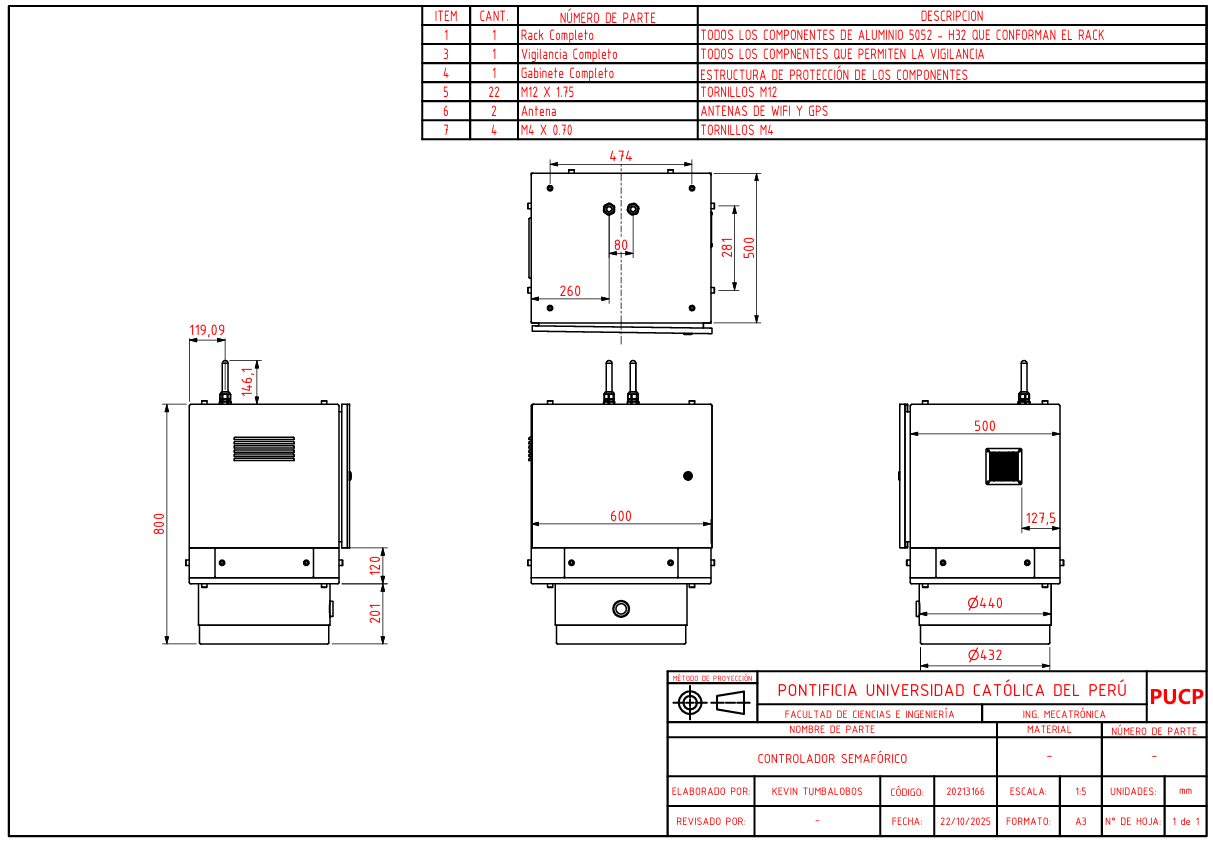
\includegraphics[width=0.97\linewidth,keepaspectratio]{media/image3.png}
\end{center}

\subsection*{G.2\quad Estructura interna: rack DIN, rieles y bases (Sección E)}
\begin{center}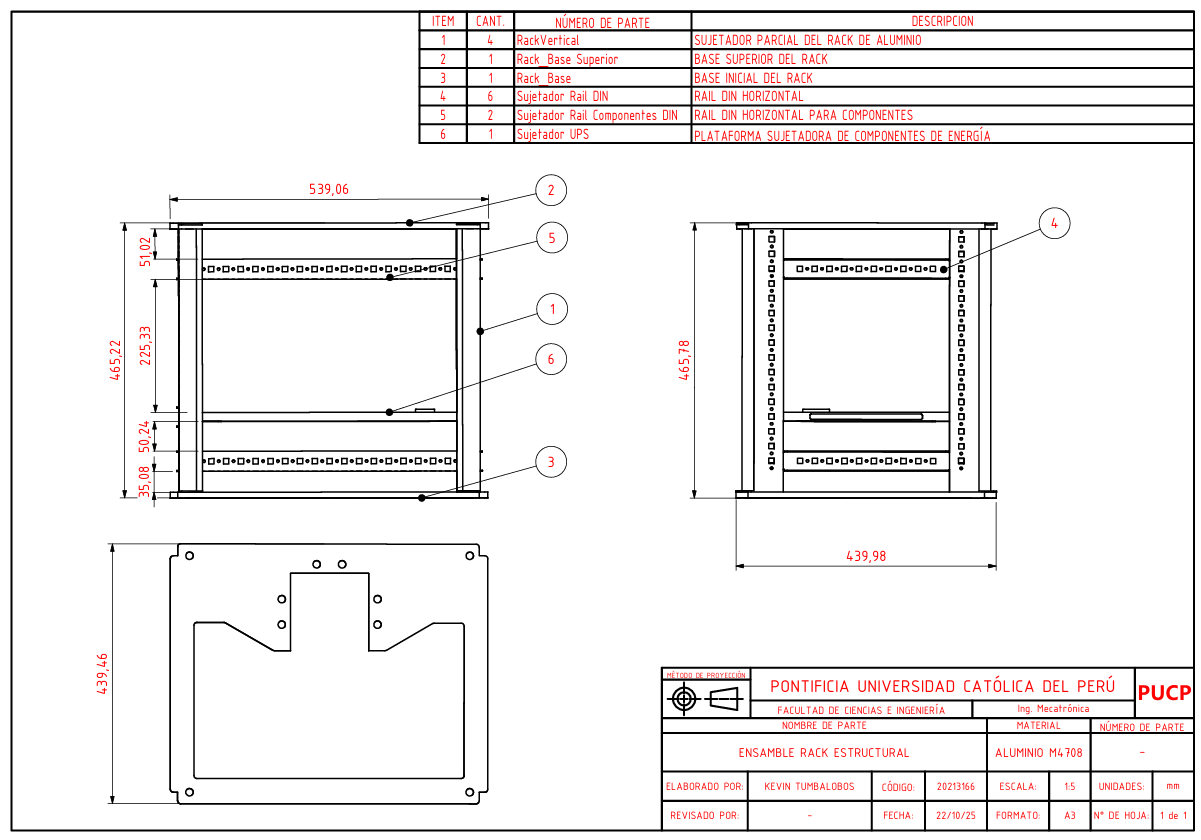
\includegraphics[width=0.97\linewidth,keepaspectratio]{media/image138.png}\end{center}
\begin{center}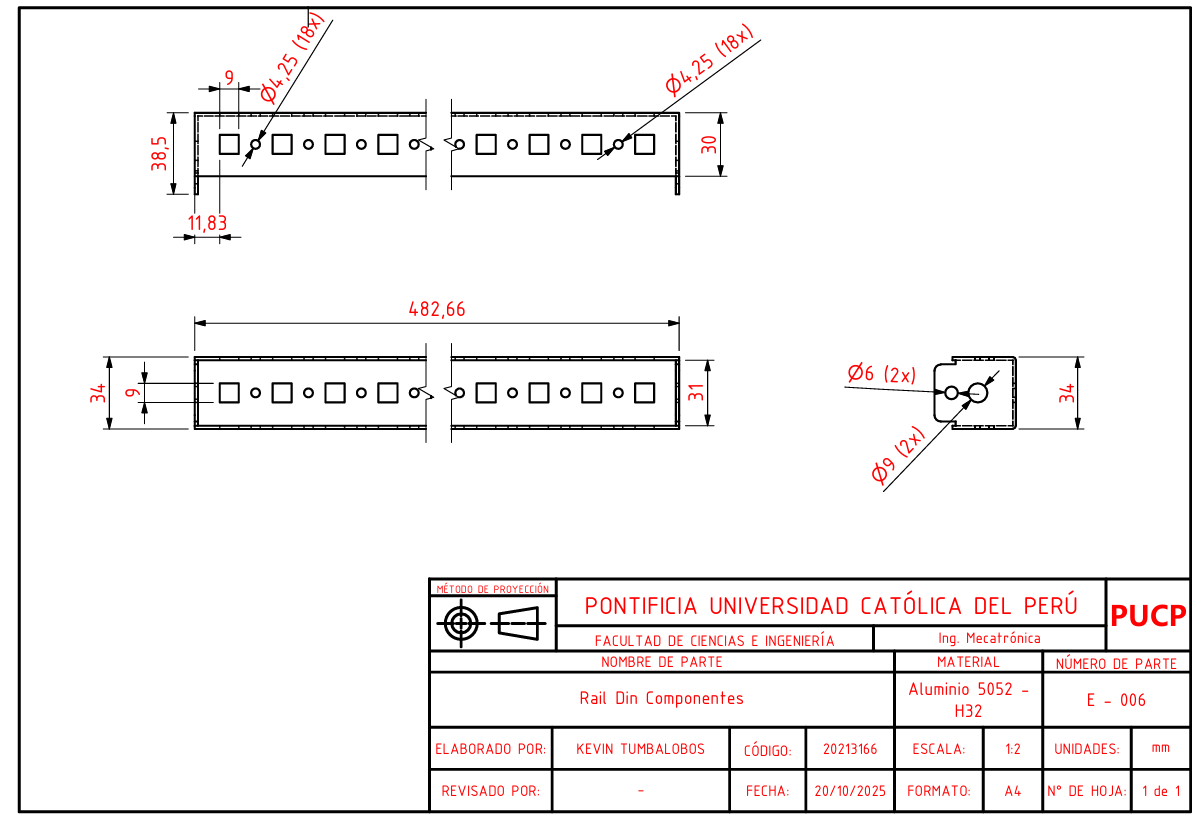
\includegraphics[width=0.97\linewidth,keepaspectratio]{media/image94.png}\end{center}
\begin{center}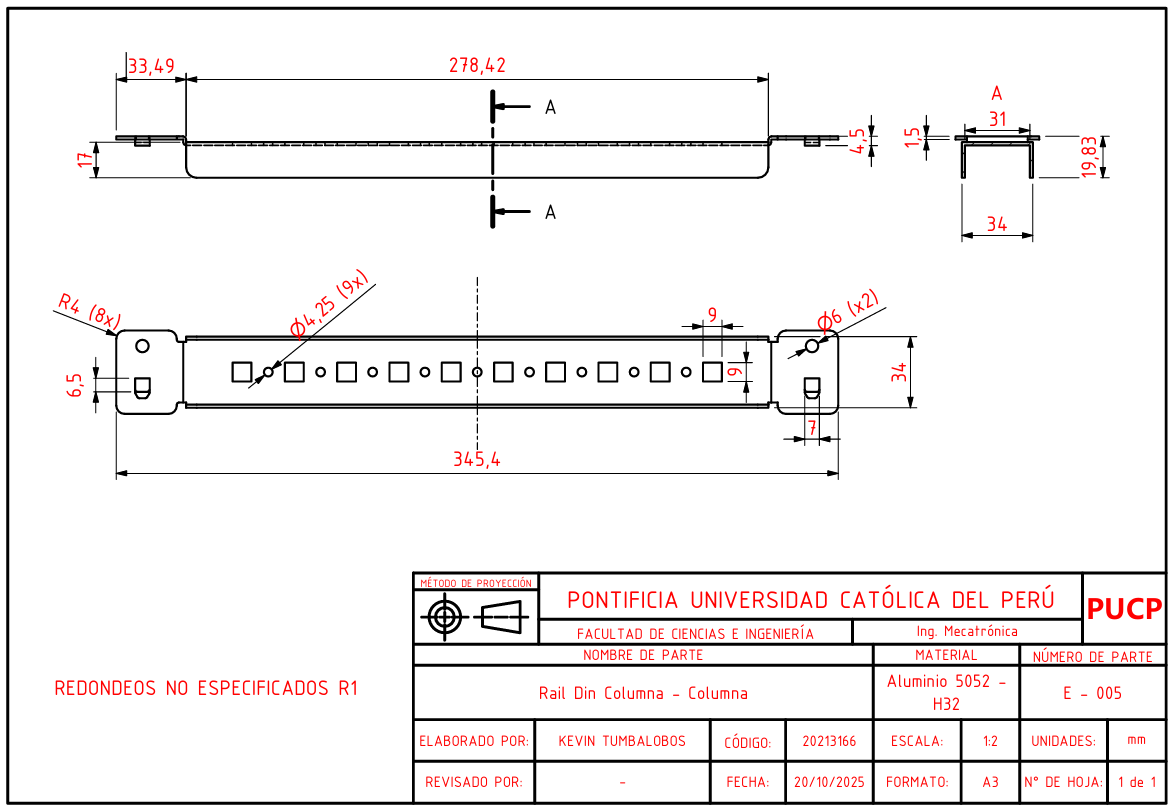
\includegraphics[width=0.97\linewidth,keepaspectratio]{media/image62.png}\end{center}
\begin{center}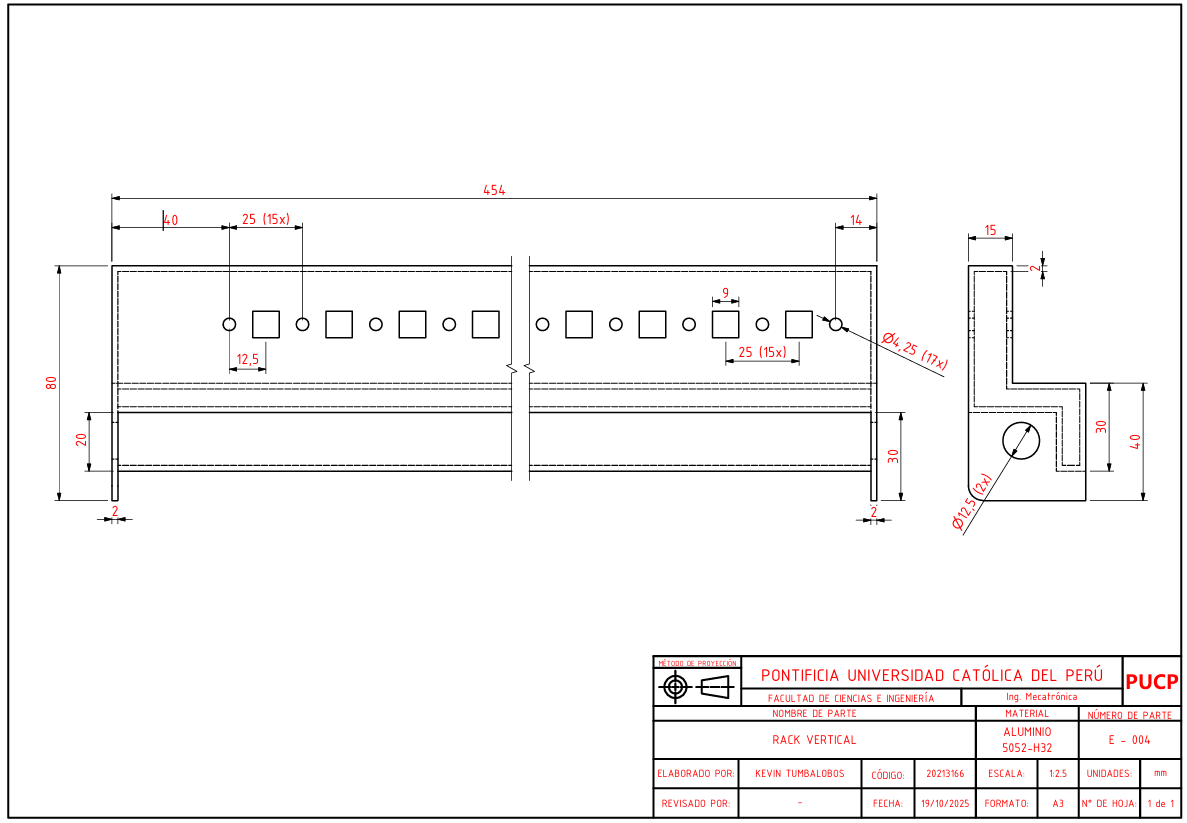
\includegraphics[width=0.97\linewidth,keepaspectratio]{media/image137.png}\end{center}
\begin{center}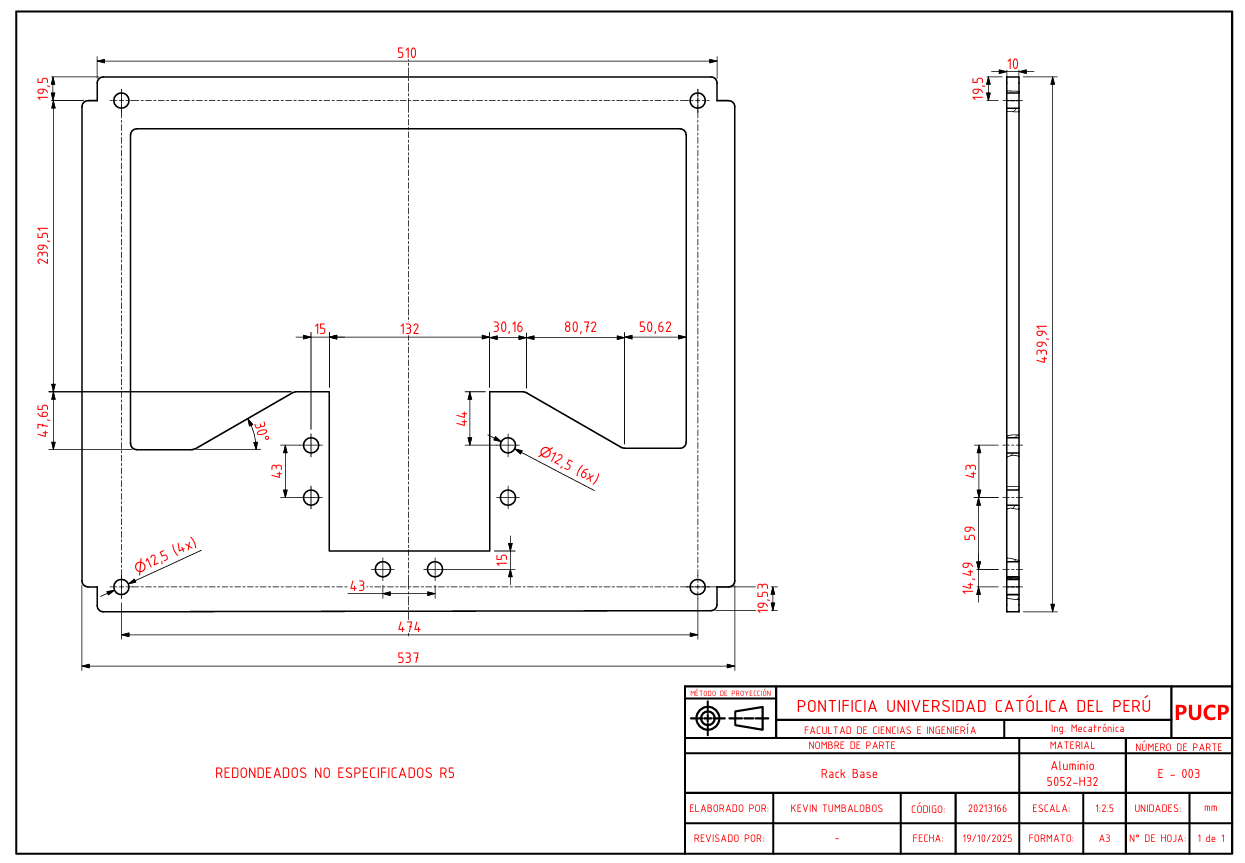
\includegraphics[width=0.97\linewidth,keepaspectratio]{media/image32.png}\end{center}
\begin{center}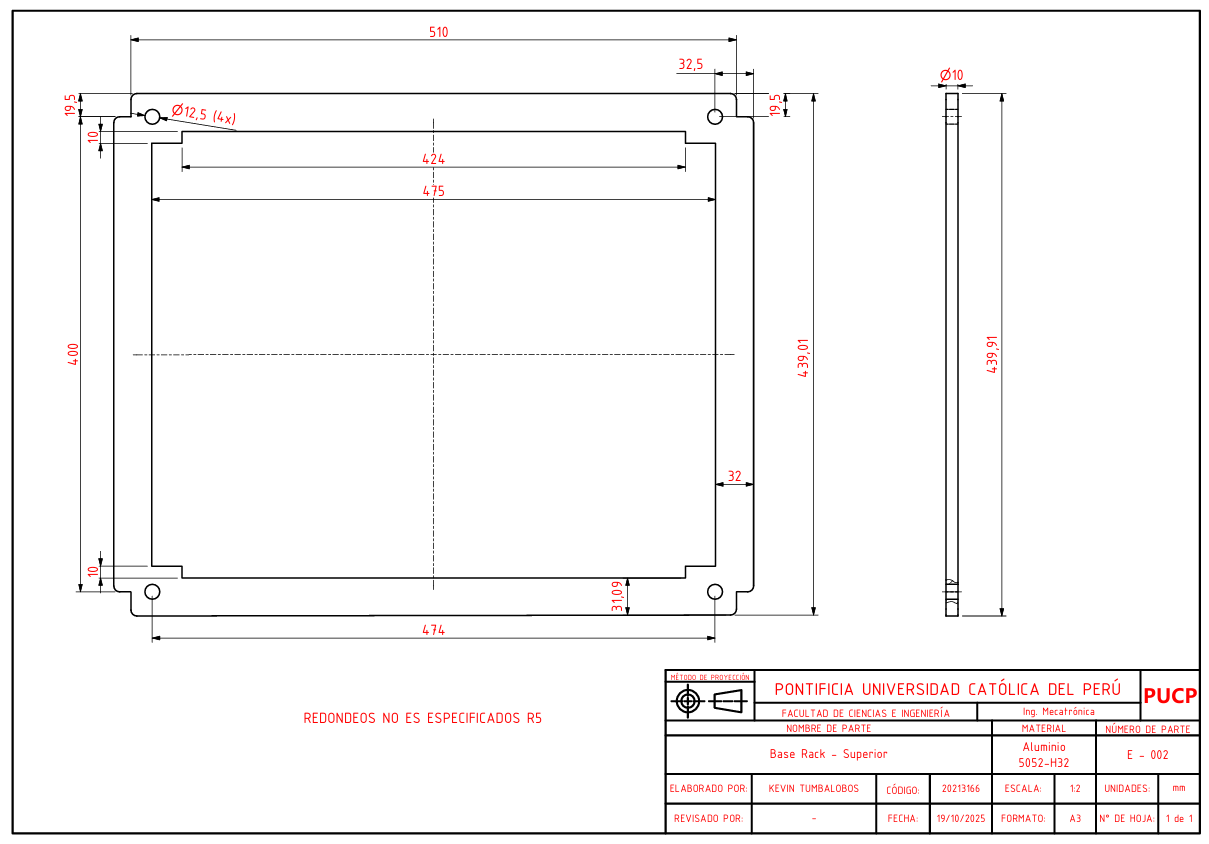
\includegraphics[width=0.97\linewidth,keepaspectratio]{media/image121.png}\end{center}
\begin{center}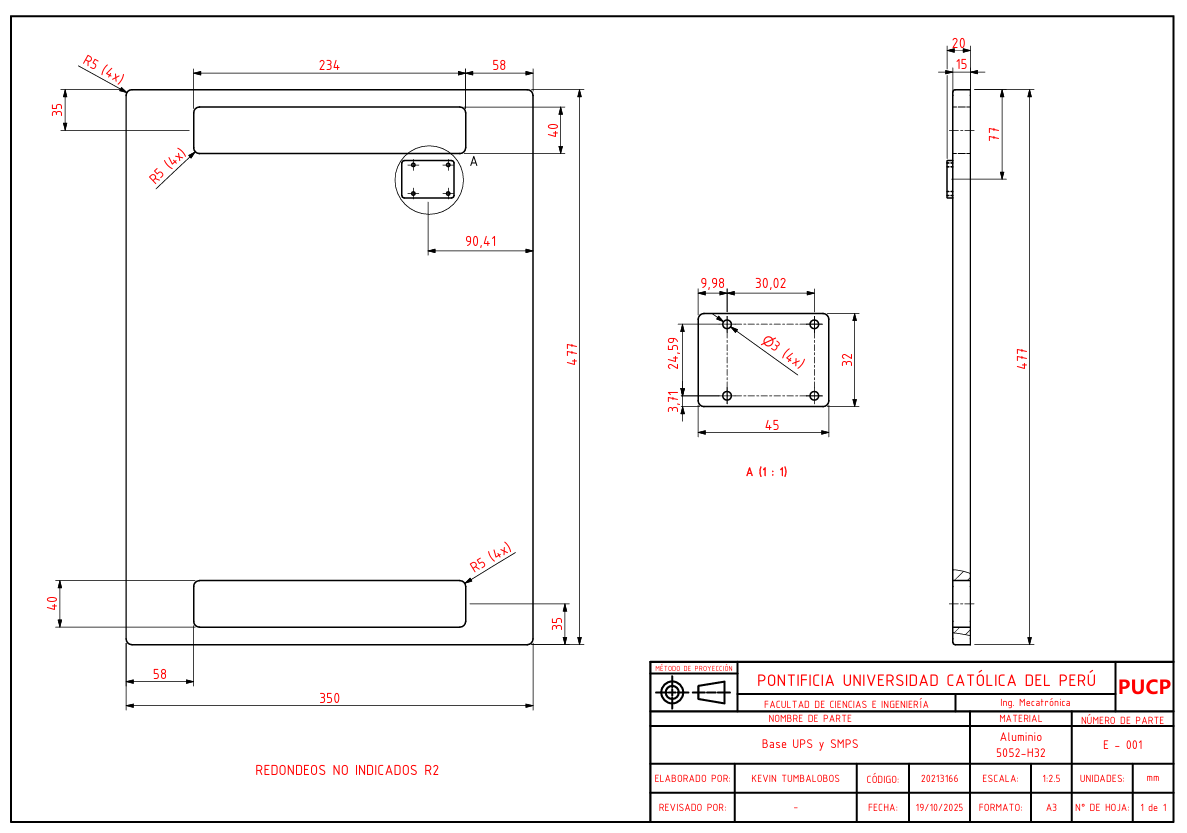
\includegraphics[width=0.97\linewidth,keepaspectratio]{media/image59.png}\end{center}

\subsection*{G.3\quad Gabinete (Sección G)}
\begin{center}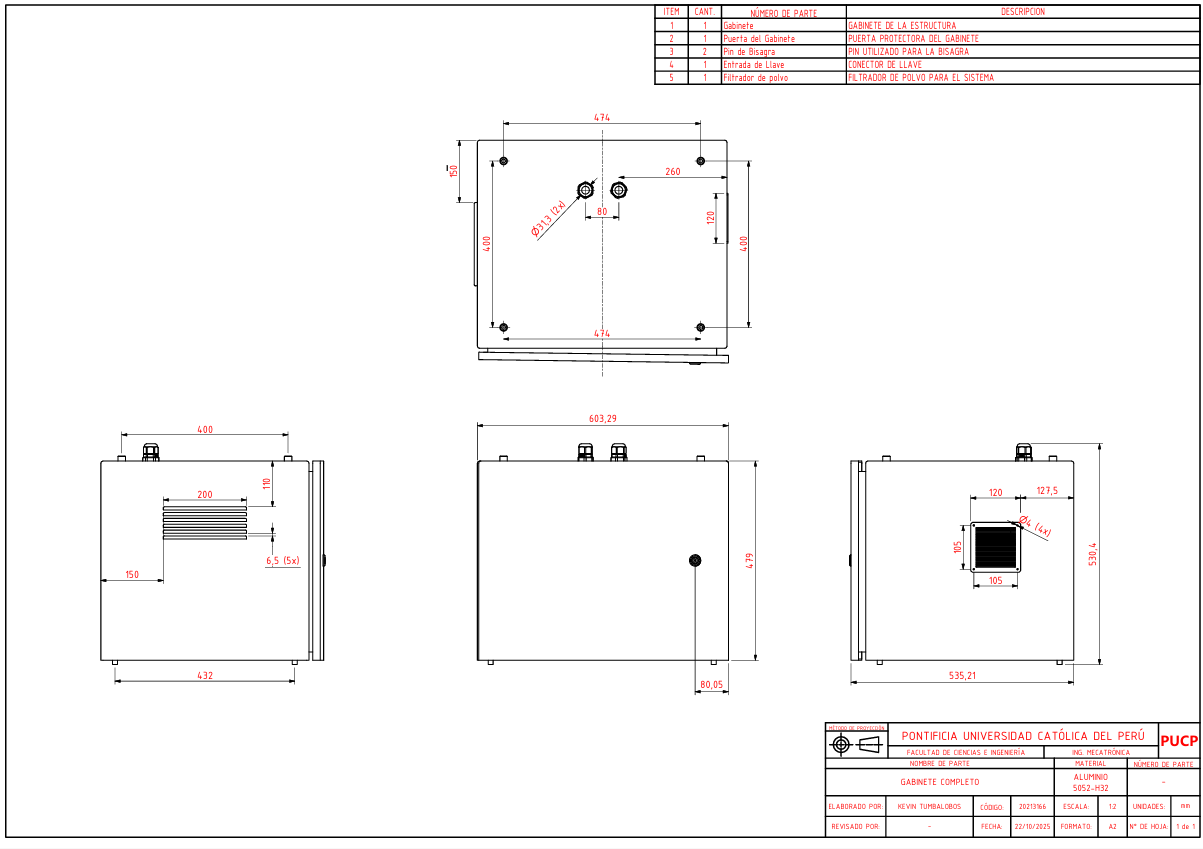
\includegraphics[width=0.97\linewidth,keepaspectratio]{media/image34.png}\end{center}
\begin{center}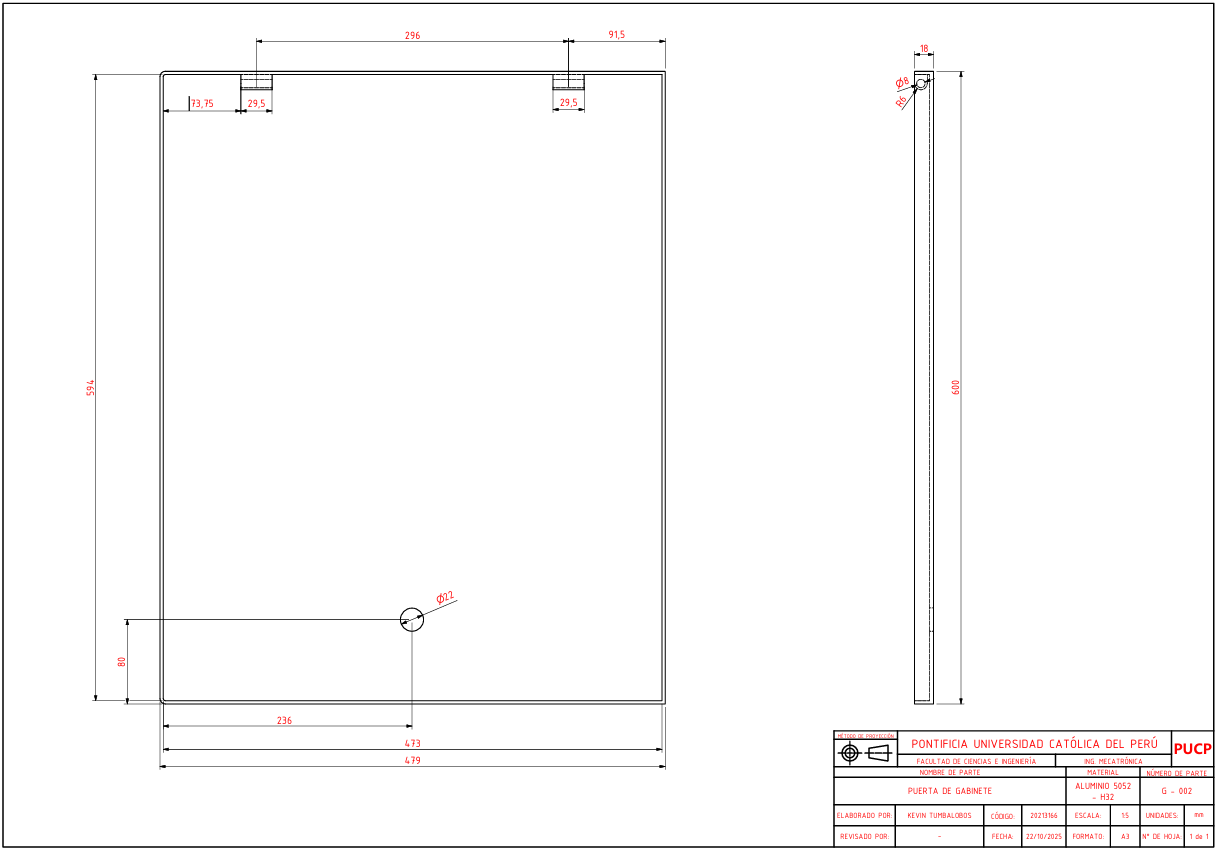
\includegraphics[width=0.97\linewidth,keepaspectratio]{media/image23.png}\end{center}
\begin{center}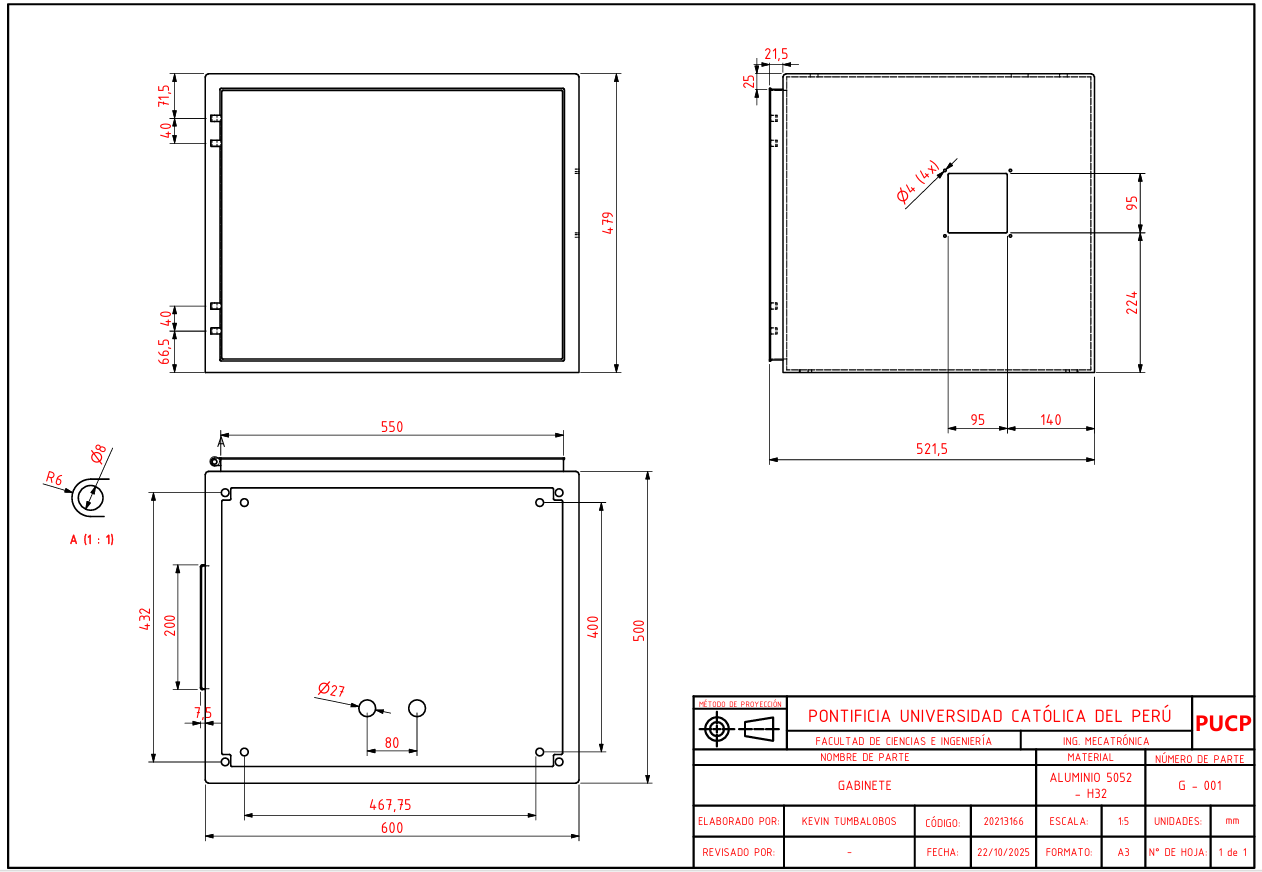
\includegraphics[width=0.97\linewidth,keepaspectratio]{media/image142.png}\end{center}

\subsection*{G.4\quad Mecanismo de orientación de la cámara (Sección M)}
\begin{center}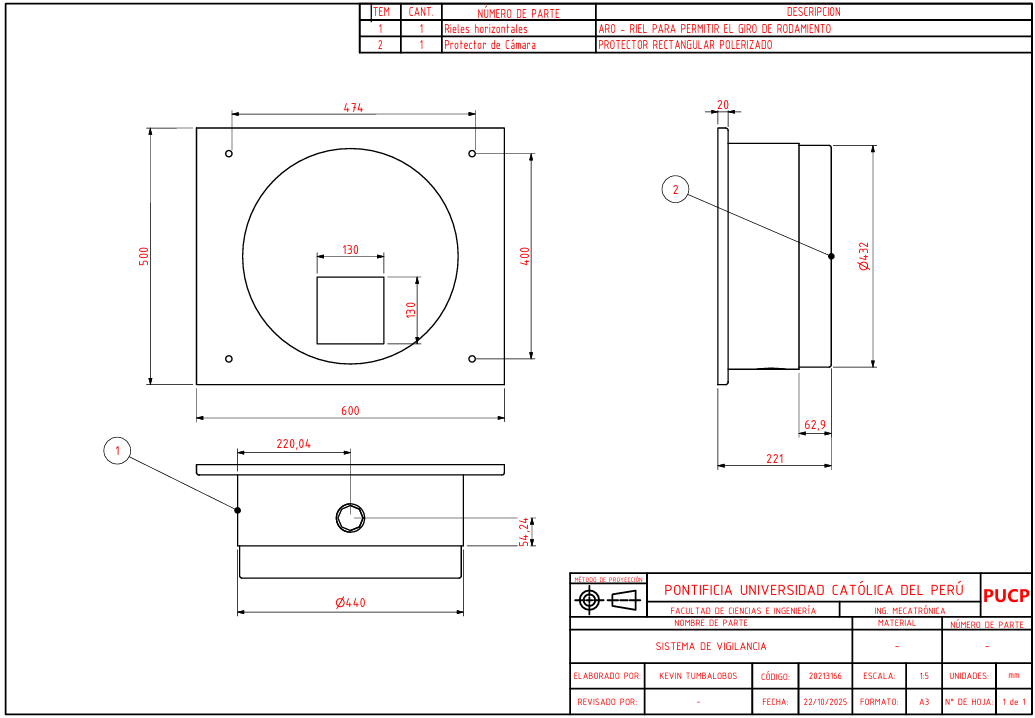
\includegraphics[width=0.97\linewidth,keepaspectratio]{media/image135.png}\end{center}
\begin{center}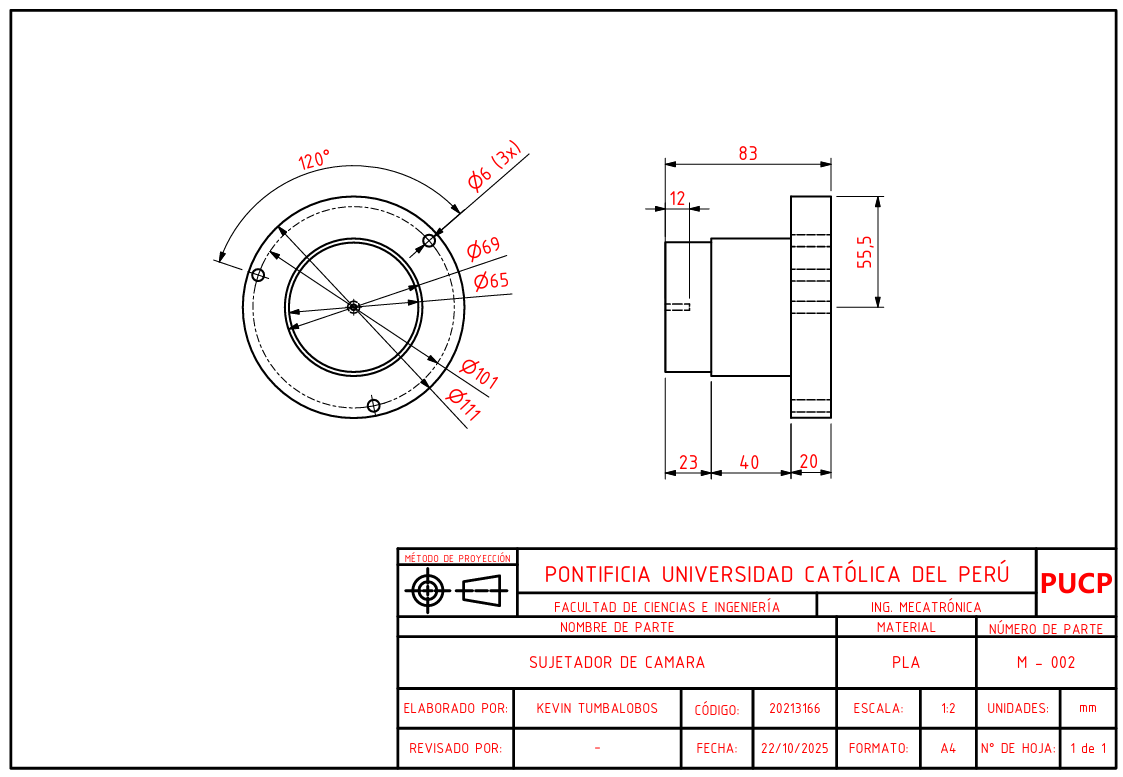
\includegraphics[width=0.97\linewidth,keepaspectratio]{media/image98.png}\end{center}
\begin{center}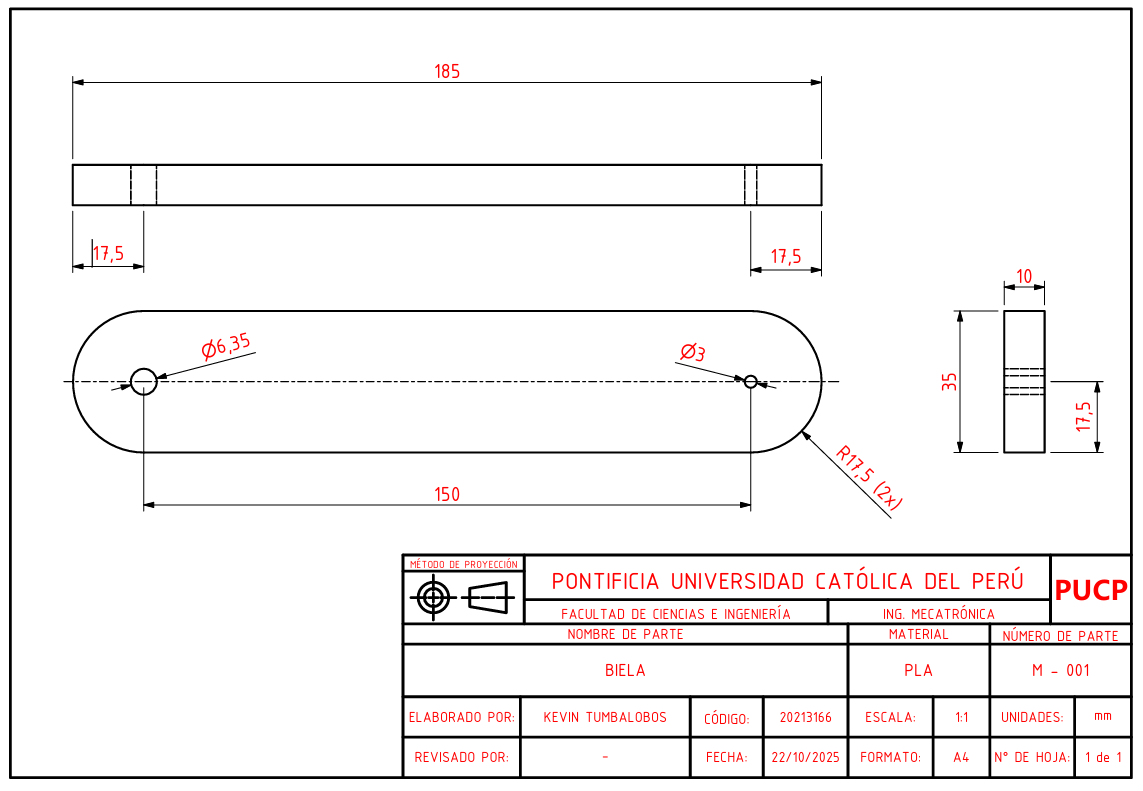
\includegraphics[width=0.97\linewidth,keepaspectratio]{media/image38.png}\end{center}
\begin{center}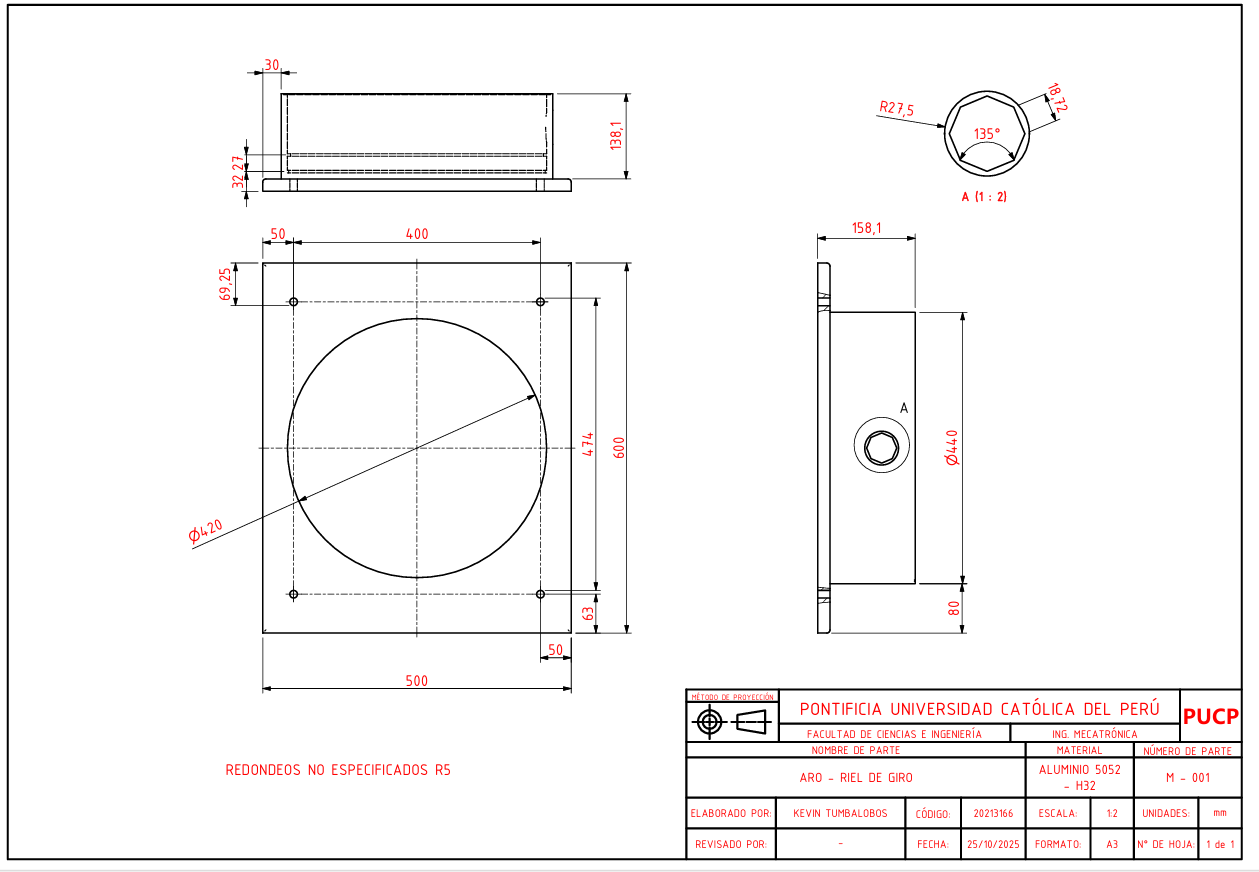
\includegraphics[width=0.97\linewidth,keepaspectratio]{media/image119.png}\end{center}

\subsection*{G.5\quad Zócalo y soporte del gabinete (Sección V)}
\begin{center}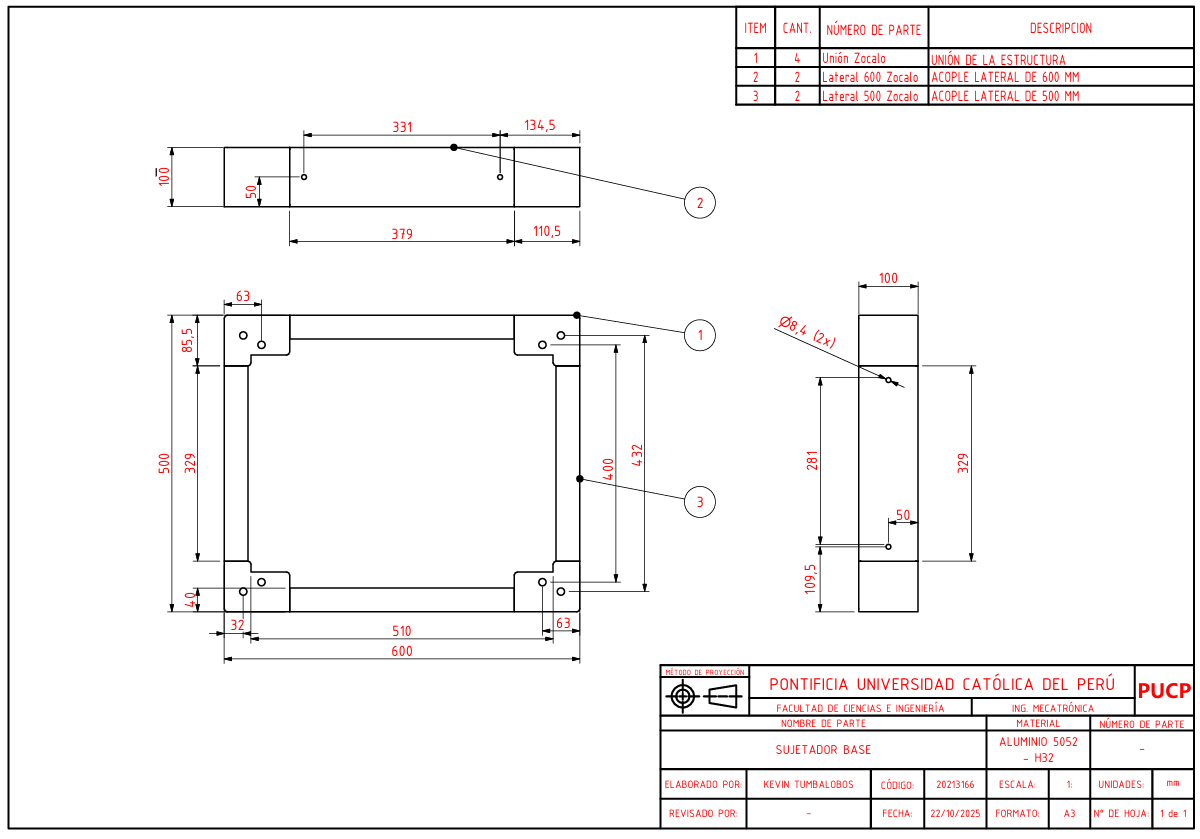
\includegraphics[width=0.97\linewidth,keepaspectratio]{media/image123.png}\end{center}
\begin{center}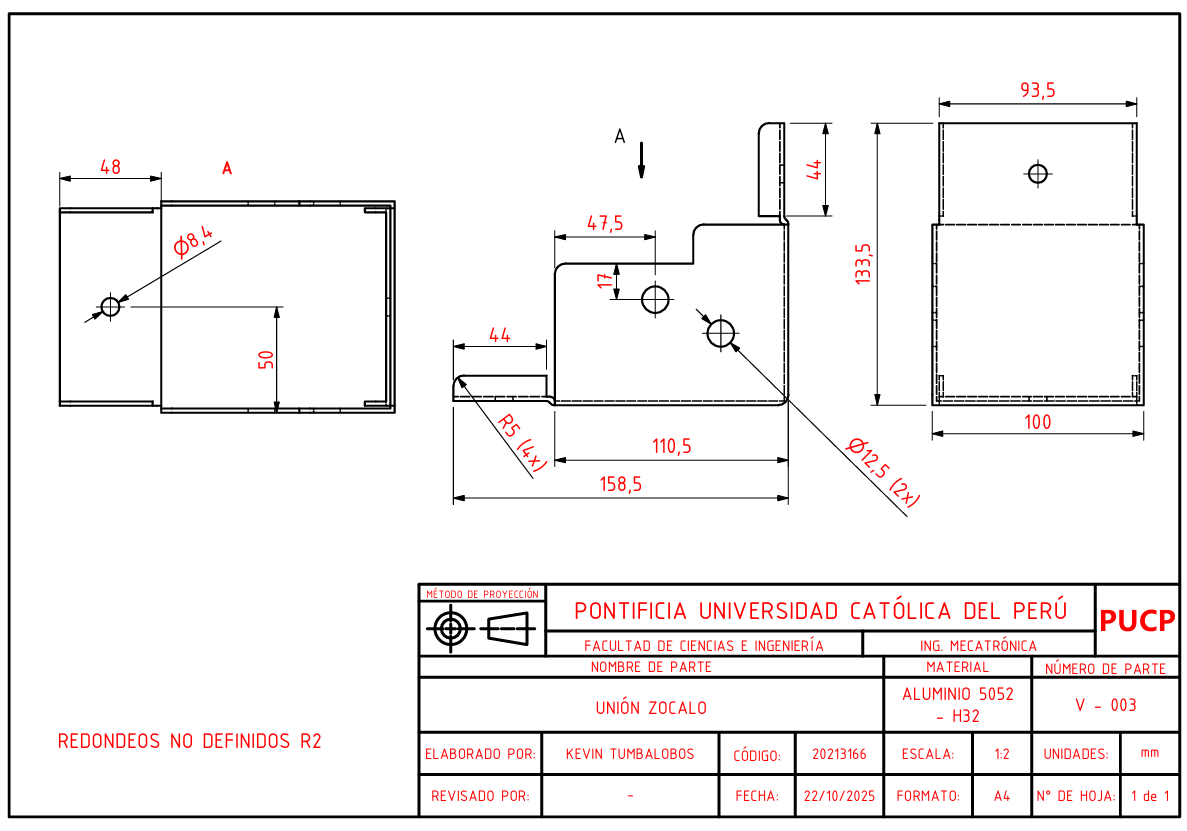
\includegraphics[width=0.97\linewidth,keepaspectratio]{media/image63.png}\end{center}
\begin{center}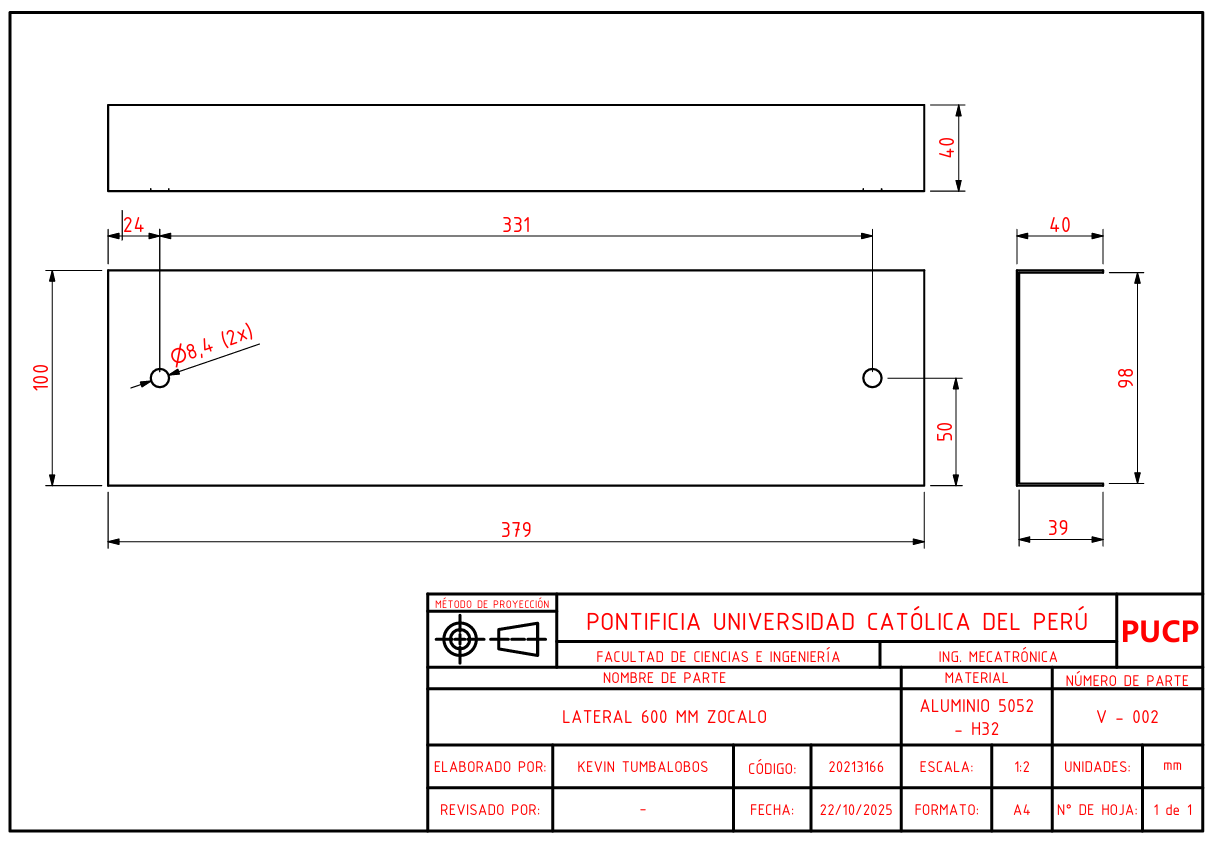
\includegraphics[width=0.97\linewidth,keepaspectratio]{media/image92.png}\end{center}
\begin{center}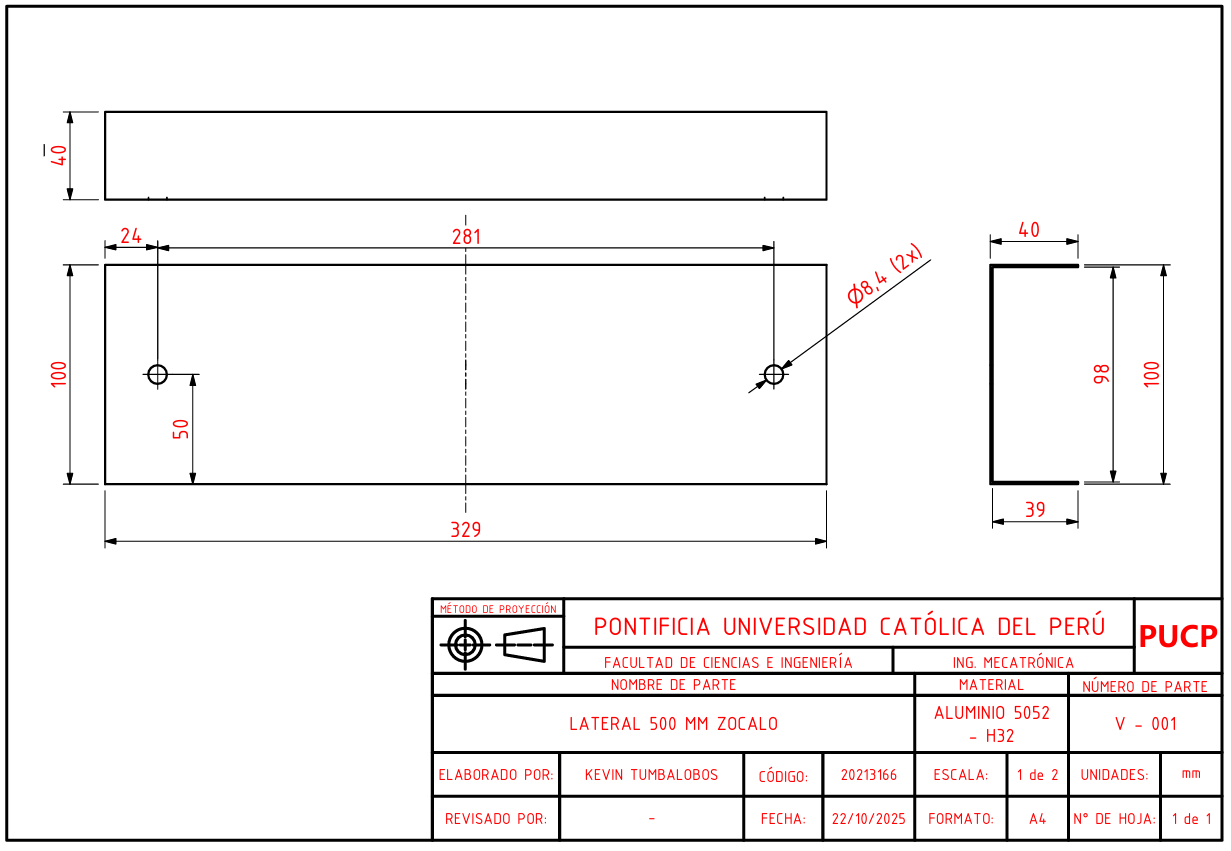
\includegraphics[width=0.97\linewidth,keepaspectratio]{media/image4.png}\end{center}

\subsection*{G.6\quad Poste metálico y placa base (Sección P)}
\begin{center}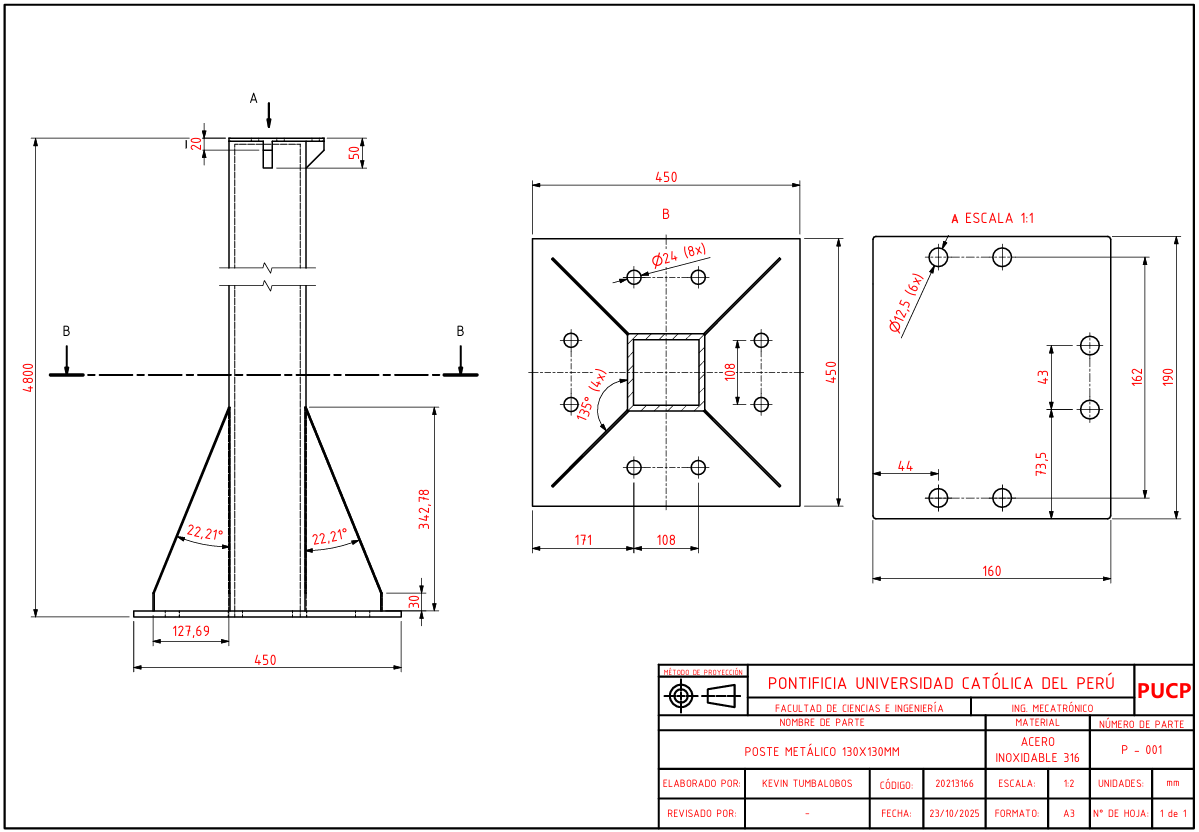
\includegraphics[width=0.97\linewidth,keepaspectratio]{media/image129.png}\end{center}

\subsection*{G.7\quad Zapata de cimentación (Sección Z)}
\begin{center}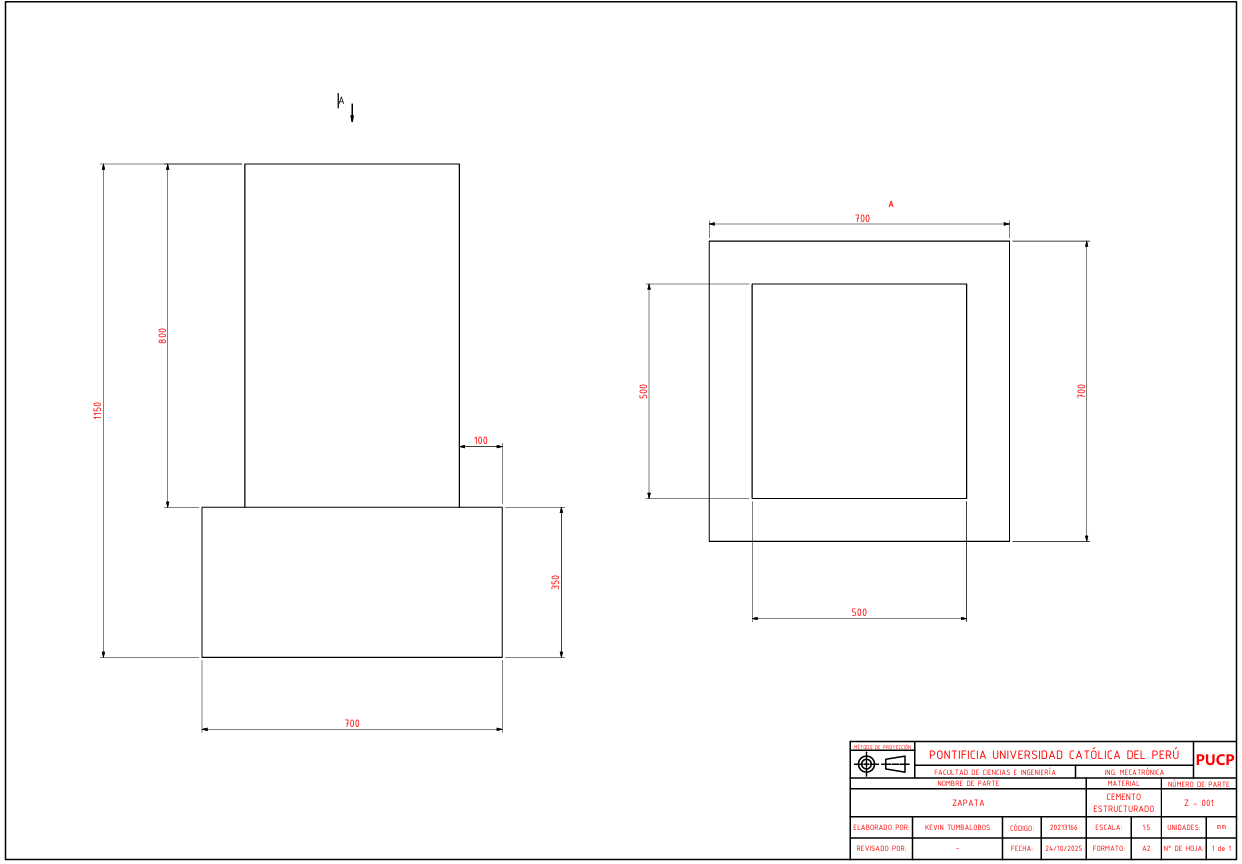
\includegraphics[width=0.97\linewidth,keepaspectratio]{media/image106.png}\end{center}

\subsection*{G.8\quad Esquemáticos electrónicos}

\begin{figure}[H]
  \centering
  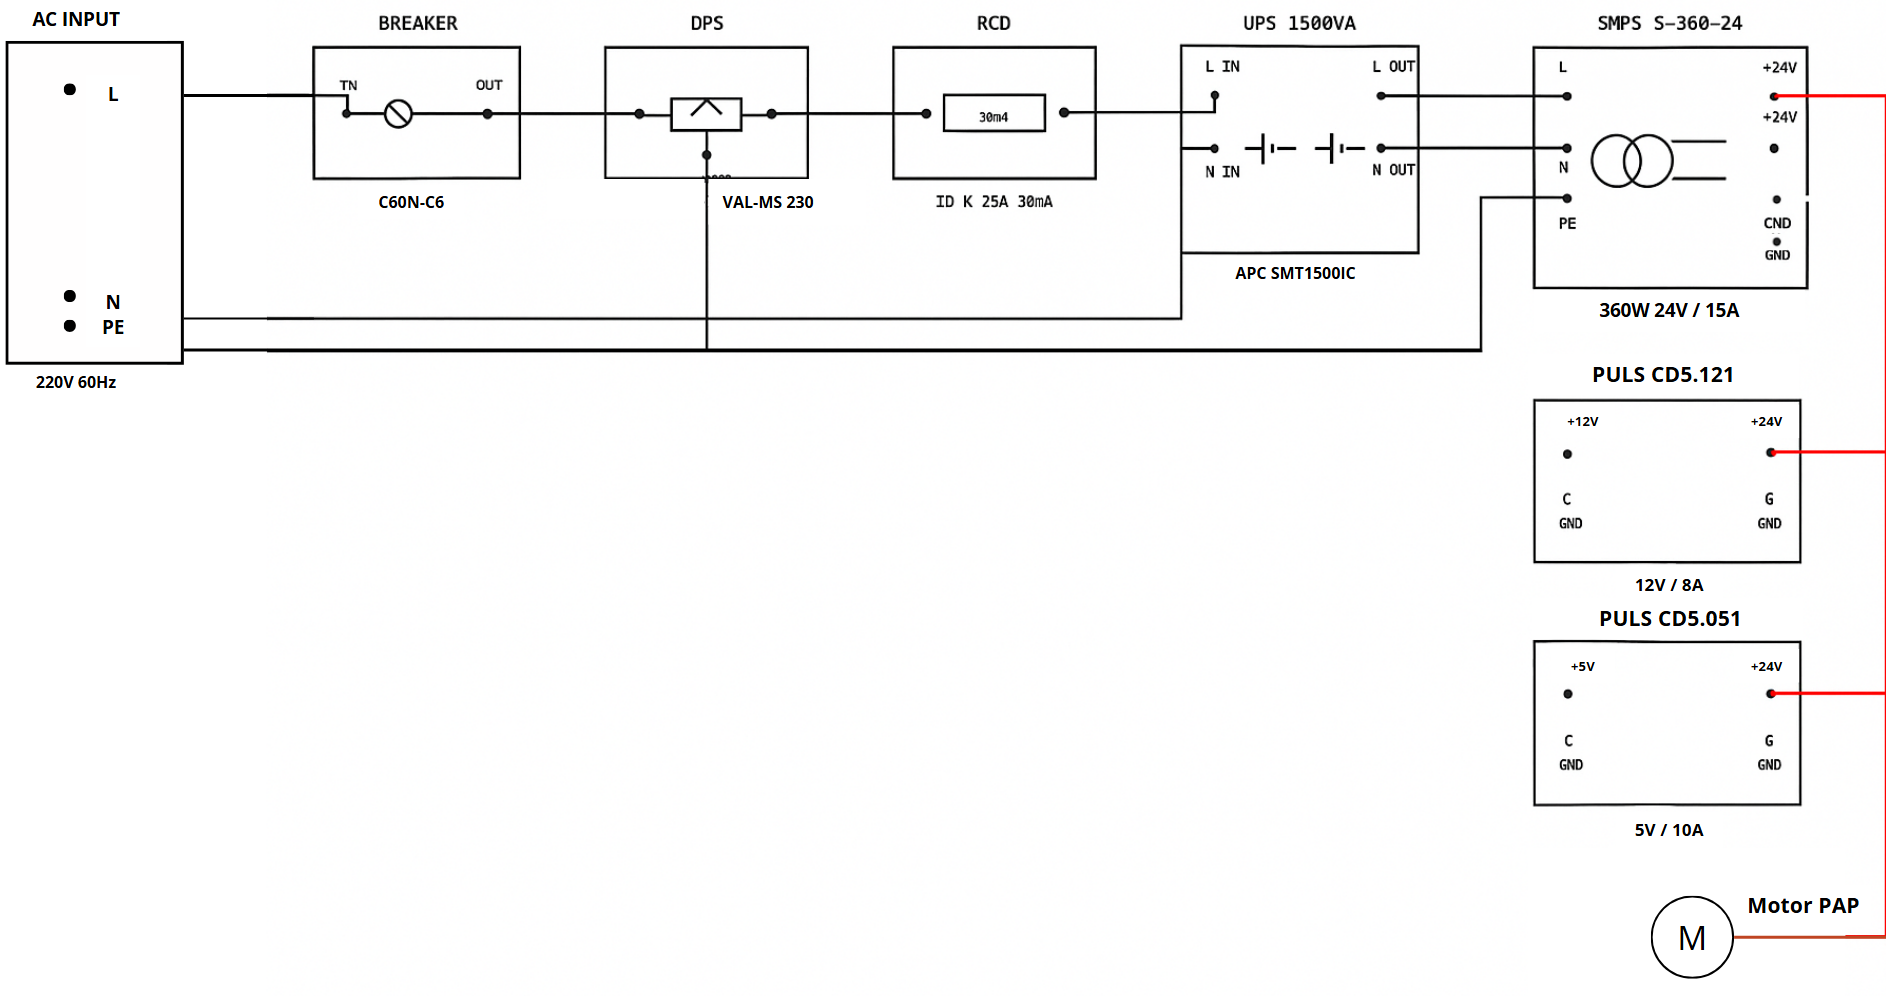
\includegraphics[width=0.85\linewidth,keepaspectratio]{media/image117.png}
  \caption{Esquemático del sistema de alimentación y protecciones.}
  \label{fig:esq-alimentacion}
  \fuente{Elaboración propia.}
\end{figure}

\begin{figure}[H]
  \centering
  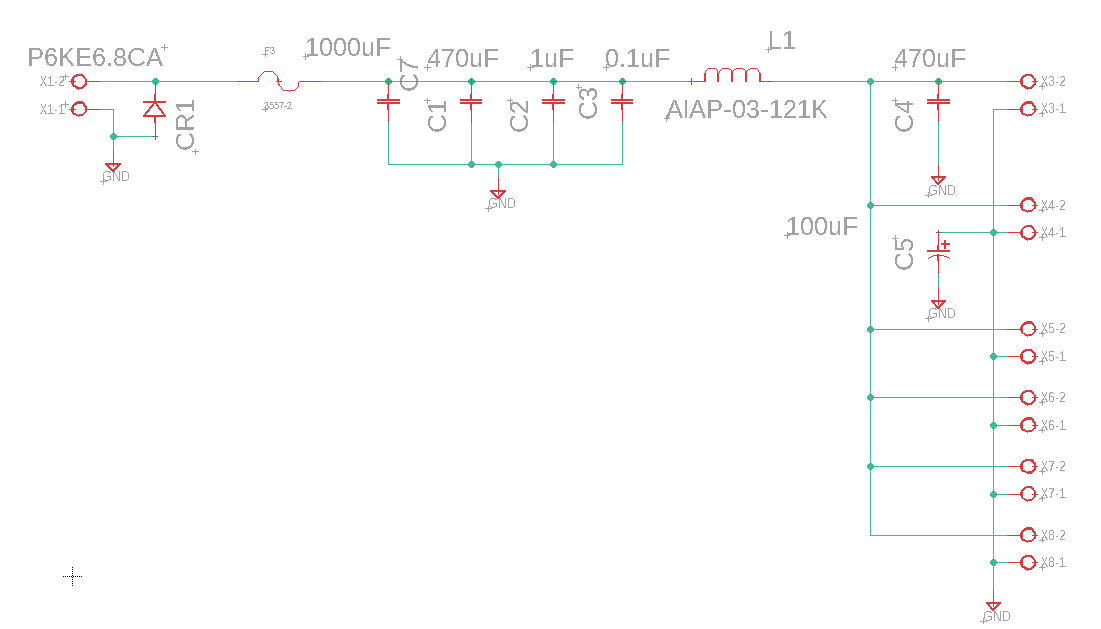
\includegraphics[width=1.0\linewidth,keepaspectratio]{media/image77.png}
  \caption{Esquemático de la línea de distribución de 5\,V.}
  \label{fig:esq-5v}
  \fuente{Elaboración propia.}
\end{figure}

\begin{figure}[H]
  \centering
  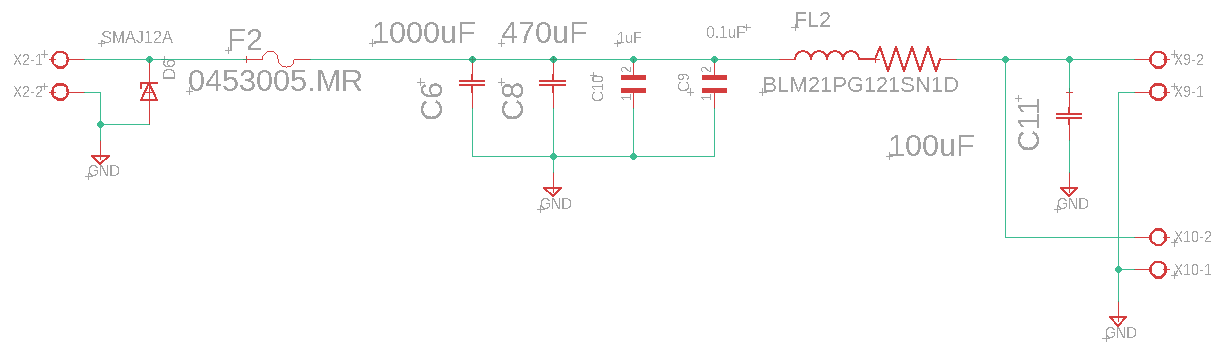
\includegraphics[width=1.0\linewidth,keepaspectratio]{media/image69.png}
  \caption{Esquemático de la línea de distribución de 12\,V.}
  \label{fig:esq-12v}
  \fuente{Elaboración propia.}
\end{figure}

\subsection*{G.9\quad Vistas complementarias del análisis estructural (FEA)}

\begin{figure}[H]
  \centering
  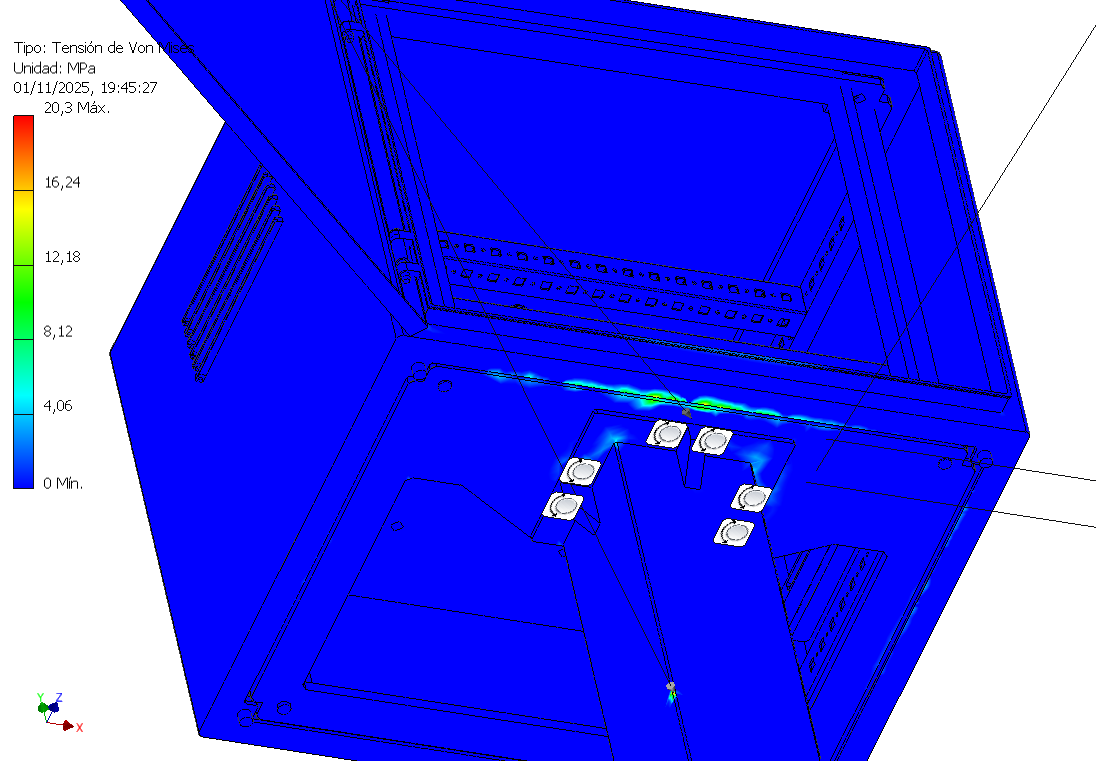
\includegraphics[width=0.55\linewidth,keepaspectratio]{media/image31.png}
  \caption{Tensión de Von Mises, vista inferior del gabinete.}
  \label{fig:vm-inferior}
  \fuente{Elaboración propia.}
\end{figure}

\begin{figure}[H]
  \centering
  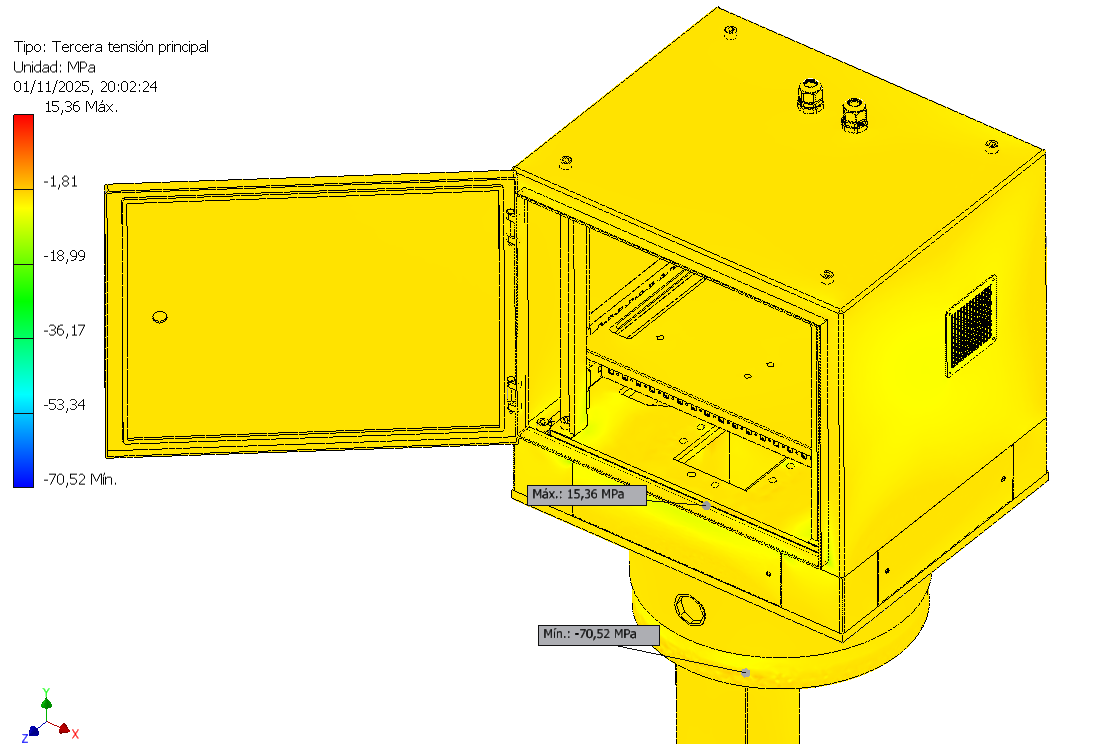
\includegraphics[width=0.6\linewidth,keepaspectratio]{media/image141.png}
  \caption{Distribución de la tercera tensión principal.}
  \label{fig:tension-p3}
  \fuente{Elaboración propia.}
\end{figure}

\begin{figure}[H]
  \centering
  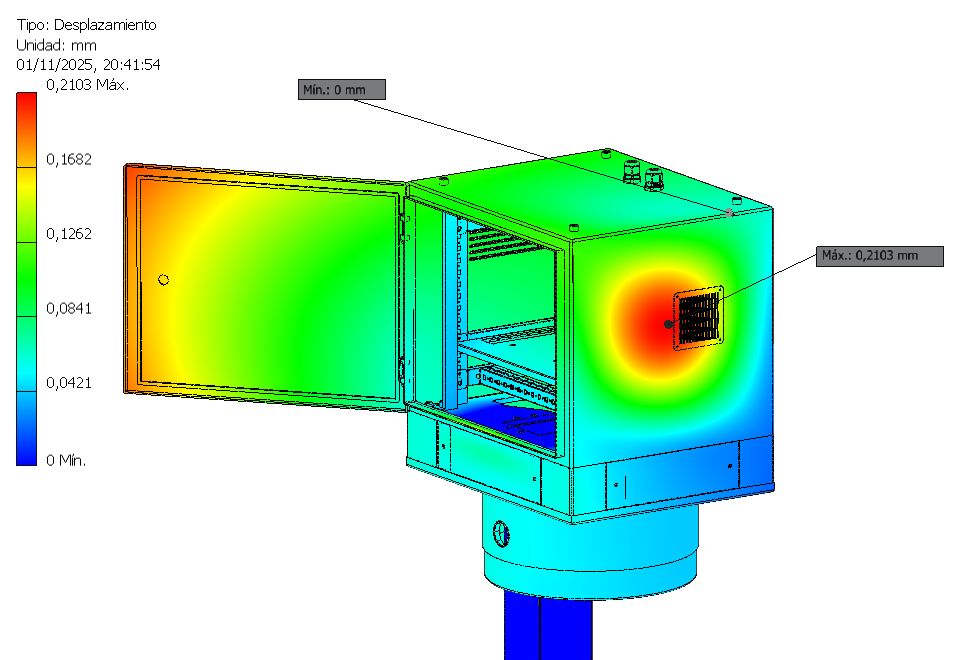
\includegraphics[width=0.7\linewidth,keepaspectratio]{media/image99.png}
  \caption{Desplazamientos en el gabinete.}
  \label{fig:desplazamiento-gabinete}
  \fuente{Elaboración propia.}
\end{figure}

\begin{figure}[H]
  \centering
  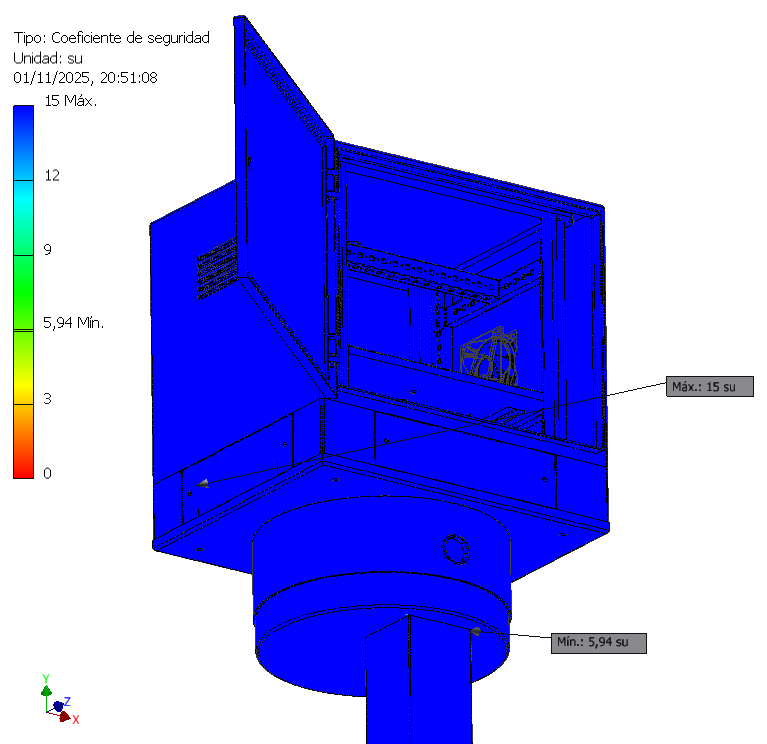
\includegraphics[width=0.8\linewidth,keepaspectratio]{media/image1.png}
  \caption{Factor de seguridad enfocado en el gabinete.}
  \label{fig:fs-gabinete}
  \fuente{Elaboración propia.}
\end{figure}

\endgroup

% ======================================================================
%                          BIBLIOGRAFÍA
% ======================================================================
\chapter*{BIBLIOGRAFÍA}\addcontentsline{toc}{chapter}{BIBLIOGRAFÍA}\label{bibliografia}
\begin{enumerate}
\def\labelenumi{\arabic{enumi}.}
\item
  Adafruit Industries. (2016, 9 de febrero). MCP3008 \textbar{} Raspberry Pi Analog to Digital Converters. \url{https://learn.adafruit.com/raspberry-pi-analog-to-digital-converters/mcp3008}
\item
  AdvancedPCB. (2024, 6 de agosto). Understanding High-Power PCB Requirements. \url{https://www.advancedpcb.com/en-us/resources/blog/understanding-high-power-pcb-requirements/}
\item
  Akçelik, R. (1981). \emph{Traffic signals: Capacity and timing analysis} (Australian Road Research Board Research Report ARR 123). Australian Road Research Board.
\item
  Aleko, D. R., \& Djahel, S. (2023). An IoT enabled traffic light controllers synchronization method for road traffic congestion mitigation. Proceedings of the 2nd International Conference on Edge Computing and Applications (ICECAA 2023), IEEE Xplore Part Number: CFP23BV8-ART. \url{https://ieeexplore.pucp.elogim.com/stamp/stamp.jsp?tp=&arnumber=9071667}
\item
  Ali, M. E. M., Durdu, A., Celtek, S. A., \& Yilmaz, A. (2021). An adaptive method for traffic signal control based on fuzzy logic with Webster and modified Webster formula using SUMO traffic simulator. \emph{IEEE Access, 9}, 102985--102997. \url{https://doi.org/10.1109/ACCESS.2021.3094270}
\item
  Altium. (2022, 10 de diciembre). IPC-2221 Calculator for PCB Trace Current and Heating. \url{https://resources.altium.com/p/ipc-2221-calculator-pcb-trace-current-and-heating}
\item
  Analog Devices. (2015). DS18B20: Programmable resolution 1-Wire digital thermometer {[}Hoja de datos{]}. \url{https://www.analog.com/media/en/technical-documentation/data-sheets/ds18b20.pdf}
\item
  APC Guard. (s.f.). Smart-UPS SMT1500IC Datasheet. \url{https://www.apcguard.com.au/datasheets/Smart-UPS_SMT1500IC.pdf}
\item
  Apolitical. (2019). Pittsburgh reduce el tiempo de viaje en un 25\% con semáforos inteligentes. \url{https://apolitical.co/solution-articles/es/pittsburgh-reduce-el-tiempo-de-viaje-25-semaforos-inteligentes}
\item
  Arshon Technology. (2025, 5 de abril). Understanding the IPC-2221 Standard: A Foundation for Reliable PCB Design. \url{https://arshon.com/blog/understanding-the-ipc-2221-standard-a-foundation-for-reliable-pcb-design/}
\item
  Asad, B., Saxena, N., \& Katos, V. (2020). Análisis de los riesgos y desafíos de seguridad y privacidad en el sistema de semáforos inteligentes en ciudades inteligentes. Cardiff University. \url{https://orca.cardiff.ac.uk/id/eprint/135436/1/IoT%20paper-Final.pdf}
\item
  Atlas Steels. (2021). \emph{Aluminium alloy 5052 data sheet}. Atlas Steels Technical Department. \url{https://www.atlassteels.com.au/}
\item
  ATO. (2020). NEMA 23 stepper motor specifications {[}Hoja de datos{]}. \url{https://www.ato.com/Content/doc/nema-23-stepper-motor-specs.pdf}
\item
  Autoridad de Transporte Urbano para Lima y Callao (ATU). (2024). \emph{Características y funcionalidades técnicas de los dispositivos de monitoreo inalámbrico (GPS) para el transporte público} (Resolución Directoral N.º D-000008-2024-ATU/DIR). Diario Oficial El Peruano. \url{https://www.elperuano.pe/noticia/236055-atu-aprueba-caracteristicas-del-monitoreo-inalambrico-gps-en-el-transporte-urbano}
\item
  Balasubramanian, S. B., Balaji, P., Munshi, A., Almukadi, W., Prabhu, T. N., K, V., \& Abouhawwash, M. (2023). Machine learning based IoT system for secure traffic management and accident detection in smart cities. PeerJ Computer Science, 9, e1259. \url{https://pmc.ncbi.nlm.nih.gov/articles/PMC10280433/}
\item
  Banco Mundial. (2024, 15 de octubre). Modernizing traffic management in Lima with World Bank support. \url{https://www.bancomundial.org/es/news/press-release/2024/10/15/modernizing-traffic-management-in-lima-with-world-bank-support}
\item
  Banks, A., \& Gupta, R. (Eds.). (2014). \emph{MQTT Version 3.1.1} (OASIS Standard). OASIS. \url{http://docs.oasis-open.org/mqtt/mqtt/v3.1.1/os/mqtt-v3.1.1-os.html}
\item
  BBMLED. (s.f.). How IoT enhances smart traffic light systems. \url{https://www.bbmled.com/es/a-news-how-iot-enhances-smart-traffic-light-systems}
\item
  BC Robotics. (s.f.). Getting Started With The Raspberry Pi 16 Channel ADC HAT. \url{https://bc-robotics.com/tutorials/getting-started-raspberry-16-channel-adc-hat/?srsltid=AfmBOoo5UNInhCebqc6AE-9IB_Cp4DineEsyD8XHiTWDtIY1t7zUg1Ld}
\item
  Bedoya Reyes, A. (2013). Anexo A: Descripción de simuladores de tráfico {[}Archivo PDF{]}. Universidad de Zaragoza. \url{https://zaguan.unizar.es/record/12971/files/TAZ-TFM-2013-1124_ANE.pdf}
\item
  Bitdefender. (2020, 20 de octubre). More than 150,000 traffic lights in the US have a critical vulnerability. \url{https://www.bitdefender.com/en-us/blog/hotforsecurity/more-than-150-000-traffic-lights-in-the-us-have-a-critical-vulnerability}
\item
  Boaz, R. W. (2009). NTCIP Center-To-Field Step by Step. Pillar Consulting, Inc. \url{https://pillarinc.com/wp-content/uploads/2019/09/Boaz_NTCIPCenterToFieldStepByStep.pdf}
\item
  Buchanan, B. (2023, 29 de enero). Traffic light hacking. ASecuritySite: When Bob Met Alice. \url{https://medium.com/asecuritysite-when-bob-met-alice/traffic-light-hacking-99638547ca33}
\item
  Carnegie Mellon University. (2019). Traffic Moves at the Speed of Technology. \url{https://www.cmu.edu/news/stories/archives/2019/october/traffic-moves-at-speed-of-technology.html}
\item
  Coral. (s.f.). Get started with the Coral USB Accelerator. \url{https://coral.ai/docs/accelerator/get-started/#3-run-a-model-on-the-edge-tpu}
\item
  Dalal, N., \& Triggs, B. (2005). Histograms of oriented gradients for human detection. \emph{2005 IEEE Computer Society Conference on Computer Vision and Pattern Recognition (CVPR)}, 886--893. \url{https://doi.org/10.1109/CVPR.2005.177}
\item
  Diario Correo. (2020). Urge sincronizar los semáforos de Lima para agilizar tránsito. \url{https://diariocorreo.pe/edicion/lima/urge-sincronizar-los-semaforos-de-lima-para-agilizar-transito-noticia/?ref=dcr}
\item
  El Comercio. (2024). Congestión vehicular en Lima: La ciudad más lenta de América Latina con solo 1.45 km/h en hora punta. \url{https://elcomercio.pe/lima/congestion-vehicular-en-lima-la-ciudad-mas-lenta-de-america-latina-con-solo-145-kmh-en-hora-punta-trafico-caos-vehicular-ultimas-noticia/}
\item
  El Español. (2024). Un gigantesco atasco creado por hackers: así conseguirían los atacantes controlar los semáforos de una ciudad. \url{https://www.elespanol.com/omicrono/tecnologia/20240718/gigantesco-atasco-creado-hackers-conseguirian-atacantes-controlar-semaforos-ciudad/871413290_0.html}
\item
  Fehon, K. (2016). Adaptive traffic signal systems overview and recent experience. Metropolitan Transportation Commission. \url{https://mtc.ca.gov/sites/default/files/4-Adaptive_Signal_Control_-_How_Does_It_Work.pdf}
\item
  Finglai Electric. (s.f.). S-360-24 -- Switching Power Supply 24V 15A. \url{https://www.finglai.com/products/switching-power-supplies/general-switching-power-supplies/S-360/S-360-24.html}
\item
  Genders, W., \& Razavi, S. (2019). \emph{An open-source framework for adaptive traffic signal control} (arXiv:1909.00395) [Preprint]. arXiv. \url{https://arxiv.org/abs/1909.00395}
\item
  Gheorghe, C., \& Soica, A. (2025). Revolutionizing urban mobility: A systematic review of AI, IoT, and predictive analytics in adaptive traffic control systems for road networks. Electronics, 14(4), 719. \url{https://www.mdpi.com/2079-9292/14/4/719}
\item
  González, J. A., \& Rodríguez, J. L. (2013). Sistema de comunicación TCP/IP para el control de una intersección semaforizada. Tecnología y Ciencias del Agua, 4(4), 11--21. \url{https://www.scielo.org.mx/scielo.php?pid=S1405-77432013000400011&script=sci_arttext}
\item
  HandsOn Technology. (s.f.). 360W 24V 15A SMPS -- Power Supply Datasheet. \url{https://www.handsontec.com/dataspecs/power%20supply/360W-24V-15A-SMPS.pdf}
\item
  Hikvision. (2022). DS-2CE57H0T-VPITF: Turbo HD camera {[}Hoja de datos{]}. Ficha técnica del fabricante.
\item
  IPC. (2003). IPC-2221A: Generic Standard on Printed Board Design. \url{https://www-eng.lbl.gov/~shuman/NEXT/CURRENT_DESIGN/TP/MATERIALS/IPC-2221A%28L%29.pdf}
\item
  ITS Perú. (2024a). Semáforos inteligentes en San Isidro. \url{https://itsperu.org/articulos/semaforos-inteligentes-tek/}
\item
  ITS Perú. (2024b). ¿Quién o qué decide el ritmo de los semáforos en Lima?. \url{https://itsperu.org/articulos/quien-o-que-decide-el-ritmo-de-los-semaforos-en-lima/}
\item
  Jitpakdeebodin, S., \& Thongprasri, P. (2024). A simple real-time traffic light control system using PLC. 2024 12th International Electrical Engineering Congress (iEECON). \url{https://ieeexplore.pucp.elogim.com/stamp/stamp.jsp?tp=&arnumber=10537877}
\item
  Khan, A., Rahman, S. u., Ullah, F., Khattak, M. I., Bait-Suwailam, M. M., \& El Sayed, H. (2024). V2I-VTL: IoT-Enabled adaptive traffic light controller and emission reduction at intersection. PeerJ Computer Science, 10, e2507. \url{https://peerj.com/articles/cs-2507/}
\item
  Kirk, J. (2020, 8 de septiembre). Full Stop: Vulnerabilities in IoT Traffic Light Systems. DataBreachToday. \url{https://www.databreachtoday.com/full-stop-vulnerabilities-in-iot-traffic-light-systems-a-14945}
\item
  Koukol, M., Zajíčková, L., Marek, L., \& Tuček, P. (2015). Fuzzy logic in traffic engineering: A review on signal control. \emph{Mathematical Problems in Engineering, 2015}, 979160. \url{https://doi.org/10.1155/2015/979160}
\item
  KSN PCB. (s.f.). The Ultimate Guide of Mastering PCB Design Guidelines. \url{https://ksnpcb.com/the-ultimate-of-mastering-pcb-design-guidelines/}
\item
  Little Bird Electronics. (s.f.). Using a Logic-level Shifter with Raspberry Pi. \url{https://learn.littlebirdelectronics.com.au/guides/using-a-logic-level-shifter-with-raspberry-pi}
\item
  MatWeb. (2024). \emph{Aluminum 5052-H32}. MatWeb Material Property Data. \url{http://www.matweb.com/}
\item
  Mean Well. (s.f.a). HDR-15-12 -- 15W 12V DIN Rail Power Supply. \url{https://meanwell-ps.com/products/hdr-15-12}
\item
  Mean Well. (s.f.b). HDR-15 Series Power Supply. \url{https://www.meanwell.com/webapp/product/search.aspx?prod=HDR-15}
\item
  Ministerio de Transportes y Comunicaciones (MTC). (2020). \emph{Manual de Sistemas Inteligentes de Transporte para la Infraestructura Vial} (Resolución Directoral N.º 017-2020-MTC/18). Gobierno del Perú. \url{https://www.gob.pe/institucion/mtc/informes-publicaciones/286952-manual-de-sistemas-inteligentes-de-transporte-para-la-infraestructura-vial}
\item
  Mirchandani, P. B., \& Lucas, D. E. (2001). RHODES-ITMS Tempe field test project: Implementation and field testing of RHODES, a real-time traffic adaptive control system (Report No. FHWA-AZ01-447). Arizona Department of Transportation. \url{https://rosap.ntl.bts.gov/view/dot/14932}
\item
  Municipalidad Metropolitana de Lima (MML). (2022). \emph{Criterios técnicos mínimos para la implementación de equipos y sistemas de semaforización en vías de la provincia de Lima} (Decreto de Alcaldía N.º 13-2022). Diario Oficial El Peruano. \url{https://busquedas.elperuano.pe/normaslegales/aprueban-criterios-tecnicos-minimos-para-la-implementacion-decreto-de-alcaldia-no-13-2022-2121889-1/}
\item
  National Electrical Manufacturers Association (NEMA). (2021). NEMA TS 2-2021: Traffic Controller Assemblies with NTCIP Requirements (Versión 03.08). \url{https://www.nema.org/docs/default-source/standards-document-library/nema-ts-2-2021-contents-and-scopeb71294ae-eb9a-45e2-a501-e5c0672dbd6b.pdf}
\item
  Naylamp Mechatronics. (s.f.a). Conversor de nivel lógico 8ch TXS0108E. \url{https://naylampmechatronics.com/conversores-ttl/282-conversor-de-nivel-logico-8ch-txs0108e.html}
\item
  Naylamp Mechatronics. (s.f.b). Fuente de alimentación conmutada AC/DC 600W 24V 25A WODE. \url{https://naylampmechatronics.com/fuentes-switching-ac-dc/945-fuente-de-alimentacion-conmutada-acdc-600w-24v-25a-wode.html}
\item
  Naylamp Mechatronics. (s.f.c). Motor PAP stepper NEMA23 57H1876-420-8-21B. \url{https://naylampmechatronics.com/motores-pap-steppers/820-motor-pap-stepper-nema23-57h1876-420-8-21b.html}
\item
  Naylamp Mechatronics. (s.f.d). Sensor de temperatura digital DS18B20. \url{https://naylampmechatronics.com/sensores-temperatura-y-humedad/16-sensor-de-temperatura-digital-ds18b20.html}
\item
  NTCIP. (2025). \emph{NTCIP 1202: Object definitions for Actuated Traffic Signal Controller (ASC) units} [Norma técnica conjunta AASHTO/ITE/NEMA]. National Transportation Communications for ITS Protocol. \url{https://www.ntcip.org/}
\item
  Pasajero7. (2023). Semáforos inteligentes: La clave para ciudades más eficientes y seguras. \url{https://www.pasajero7.com/semaforos-inteligentes-la-clave-para-ciudades-mas-eficientes-y-seguras/}
\item
  Pi My Life Up. (2024, 25 de septiembre). Raspberry Pi ADC (Analog to Digital Converter). \url{https://pimylifeup.com/raspberry-pi-adc/}
\item
  PULS Power. (s.f.a). CD5.051 -- 5V, 10A DIN Rail Power Supply. \url{https://products.pulspower.com/en/cd5-051.html}
\item
  PULS Power. (s.f.b). CD5.121 -- 12V, 5A DIN Rail Power Supply. \url{https://products.pulspower.com/en/cd5-121.html}
\item
  Rafique, M. T., Mustafa, A., \& Sajid, H. (2024). \emph{Reinforcement learning for adaptive traffic signal control: Turn-based and time-based approaches to reduce congestion} (arXiv:2408.15751) [Preprint]. arXiv. \url{https://arxiv.org/abs/2408.15751}
\item
  Raspberry Pi Forums. (2023, 11 de marzo). Attaching 5V sensors to the Raspberry Pi?. \url{https://forums.raspberrypi.com/viewtopic.php?t=348710}
\item
  Raspberry Pi Forums. (2025, 12 de enero). Multiple HATS and extra GPIO connections on RbPi5. \url{https://forums.raspberrypi.com/viewtopic.php?t=382395}
\item
  Raspberry Pi Foundation. (2023). Compute Module 5 IO board datasheet {[}Hoja de datos{]}. \url{https://datasheets.raspberrypi.com/cm5/cm5io-datasheet.pdf}
\item
  Raspberry Pi Stack Exchange. (2014, 13 de marzo). Using 5 volts on an mcp3008. \url{https://raspberrypi.stackexchange.com/questions/14450/using-5-volts-on-an-mcp3008}
\item
  Redmon, J., Divvala, S., Girshick, R., \& Farhadi, A. (2016). You only look once: Unified, real-time object detection. \emph{2016 IEEE Conference on Computer Vision and Pattern Recognition (CVPR)}, 779--788. \url{https://doi.org/10.1109/CVPR.2016.91}
\item
  S, S., Kingslin, M. T., M, S., Sivarajan, S., Josphine, C. V., \& Lakshmi, C. K. R. (2023). IoT based on smart traffic lights and streetlight system. Proceedings of the Second International Conference on Edge Computing and Applications (ICECAA 2023), IEEE Xplore Part Number: CFP23BV8-ART. \url{https://ieeexplore.pucp.elogim.com/stamp/stamp.jsp?tp=&arnumber=10212121}
\item
  Sachan, A., \& Kumar, N. (2024). SDN-enabled quantized LQR for smart traffic light controller to optimize congestion. ACM Transactions on Internet Technology, 24(1), Article No. 7, 1-25. \url{https://acm.pucp.elogim.com/doi/10.1145/3641104}
\item
  Sacyr. (s.f.). Semáforos inteligentes para reducir la contaminación. \url{https://sacyr-pre.sacyr.com/-/semaforos-inteligentes-para-reducir-la-contaminacion}
\item
  SCATS. (s.f.). Sistema de control de semáforos. \url{https://www.scats.com.au/home}
\item
  Schneider Electric. (s.f.). APC Smart-UPS línea interactiva 1500VA, torre, 230V (SMT1500IC). \url{https://www.se.com/pe/es/product/SMT1500IC/apc-smartups-l%C3%ADnea-interactiva-1500va-torre-230v-8x-iec-c13-salidas-puerto-smartconnect+smartslot-avr-lcd/}
\item
  SciELO. (2023, julio). Tecnologías emergentes en la infraestructura vial en el contexto peruano. SciELO Perú. \url{http://www.scielo.org.pe/scielo.php?script=sci_arttext&pid=S1810-99932023000200093}
\item
  SCOOT. (s.f.). Split Cycle Offset Optimization Technique. \url{https://trlsoftware.com/software/intelligent-signal-control/scoot/}
\item
  Seeed Studio. (s.f.). Getting started with Raspberry Pi 4G LTE HAT. \url{https://wiki.seeedstudio.com/es/getting_started_raspberry_pi_4g_lte_hat/}
\item
  Sierra Circuits. (2023, 30 de enero). IPC-2221 Standards in PCB Design. \url{https://www.protoexpress.com/blog/ipc-2221-circuit-board-design/}
\item
  Sierra Circuits. (2025, 27 de enero). 7 PCB Layout Design Tips for Power Electronics. \url{https://www.protoexpress.com/blog/pcb-layout-design-tips-for-power-electronics/}
\item
  Smart Cities Dive. (2017). This AI traffic system in Pittsburgh has reduced travel time by 25\%. \url{https://www.smartcitiesdive.com/news/this-ai-traffic-system-in-pittsburgh-has-reduced-travel-time-by-25/447494/}
\item
  Smith, S. F., Barlow, G. J., Xie, X.-F., \& Rubinstein, Z. B. (2013). SURTRAC: Scalable Urban Traffic Control. The Robotics Institute, Carnegie Mellon University. \url{https://www.ri.cmu.edu/pub_files/2013/1/13-0315.pdf}
\item
  StepperOnline. (2020). DM542T digital stepping drive {[}Hoja de datos{]}. \url{https://5.imimg.com/data5/SELLER/Doc/2020/12/GL/TF/KS/16561264/stepperonline-dm542t-digital-stepping-drive.pdf}
\item
  Tario, J. D., Dillmann, R., Lardoux, J., Martinez, R., White, C., Gross, N., Patel, N., \& Meyer, R. (2014). Adaptive traffic signal control for Tarrytown Road in White Plains, New York (Final Report). Prepared for New York State Energy Research and Development Authority \& New York State Department of Transportation. TransCore ITS, LLC. \url{https://www.nyserda.ny.gov/-/media/Project/Nyserda/Files/Publications/Research/Transportation/Adaptive-Traffic-Signal-Control-Tarrytown-Road.pdf}
\item
  ThomasNet. (2025). \emph{All about 5052 aluminum (properties, strength and uses)}. Thomas Publishing Company. \url{https://www.thomasnet.com/articles/metals-metal-products/5052-aluminum/}
\item
  Trafficware. (2014). Summary of Version 8 releases. \url{https://online.trafficware.com/downloads/v8/Summary%20of%20Version%208%20Releases.pdf}
\item
  Varaiya, P. (2013). Max pressure control of a network of signalized intersections. \emph{Transportation Research Part C: Emerging Technologies, 36}, 177--195. \url{https://doi.org/10.1016/j.trc.2013.08.014}
\item
  Viola, P., \& Jones, M. (2001). Rapid object detection using a boosted cascade of simple features. \emph{2001 IEEE Computer Society Conference on Computer Vision and Pattern Recognition (CVPR)}, 511--518. \url{https://doi.org/10.1109/CVPR.2001.990517}
\item
  Webster, F. V. (1958). \emph{Traffic signal settings} (Road Research Technical Paper No.~39). Her Majesty's Stationery Office, Road Research Laboratory.
\item
  Wevolver. (2025). \emph{Selección de materiales para gabinetes electrónicos a la intemperie: aluminio frente a policarbonato}. Wevolver. \url{https://www.wevolver.com/}
\item
  Wojke, N., Bewley, A., \& Paulus, D. (2017). Simple online and realtime tracking with a deep association metric. \emph{2017 IEEE International Conference on Image Processing (ICIP)}, 3645--3649. \url{https://doi.org/10.1109/ICIP.2017.8296962}
\item
  Yalcinli, F., Akdemir, B., \& Durdu, A. (2024). Adaptive traffic management model for signalised intersections. \emph{Elektronika ir Elektrotechnika, 30}(3), 72--82. \url{https://doi.org/10.5755/j02.eie.36536}
\item
  YouTube. (2018, 8 de abril). DS18B20 digital temperature sensor tutorial {[}Video{]}. \url{https://www.youtube.com/watch?v=pxcFjBZCGtU}
\item
  YouTube. (2020, 14 de julio). Cómo conectar y usar el driver DM542T con motor NEMA 23 {[}Video{]}. \url{https://www.youtube.com/watch?v=mtWuL7NXCTA}
\item
  Zivkovic, Z. (2004). Improved adaptive Gaussian mixture model for background subtraction. \emph{Proceedings of the 17th International Conference on Pattern Recognition (ICPR)}, 28--31. \url{https://doi.org/10.1109/ICPR.2004.1333992}
\end{enumerate}

